\chapter{More benchmarking results}\label{appendix:more-benchmarking-results}
%%%%%

%%
\section{Simulations: Optimal learned window lengths}\label{appendix:sim-optimal-window-lengths}
%%


\begin{figure}[ht]
  \centering
  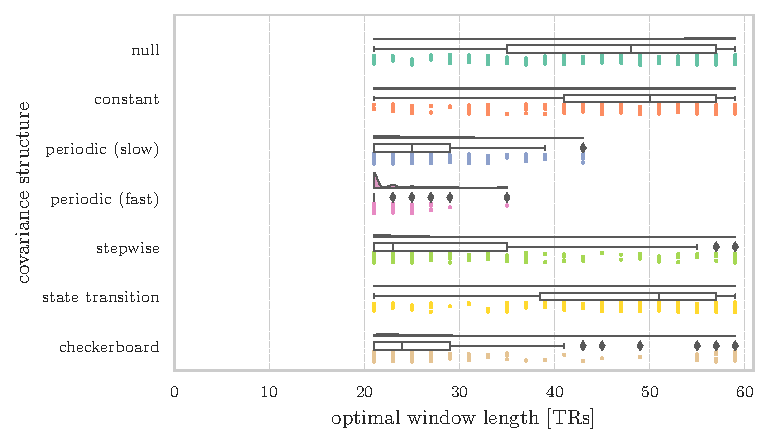
\includegraphics[width=\textwidth]{fig/sim/d2/N0120_T0200/no_noise/SW_cross_validated_optimal_window_lengths}
  \caption{
    Simulations benchmark optimal cross-validated window lengths learned from bivariate ($D = 2$) noiseless data for $N = 120$.
    Each dot represents one of $T = 200$ trials.
  }\label{fig:sim-optimal-window-lengths-N120}
\end{figure}


\begin{figure}[ht]
  \centering
  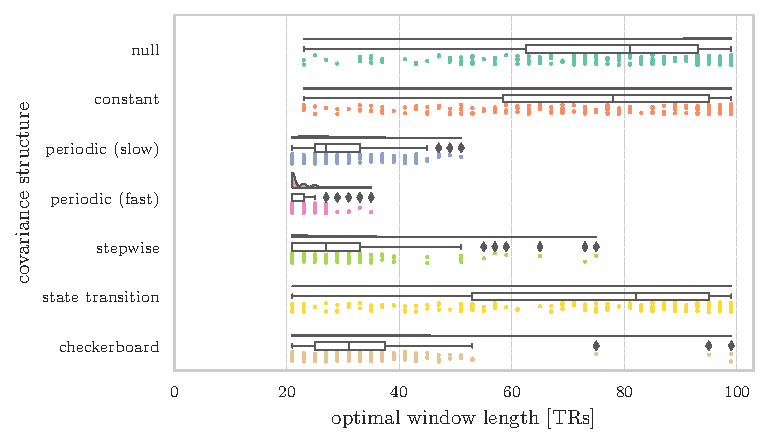
\includegraphics[width=\textwidth]{fig/sim/d2/N0200_T0200/no_noise/SW_cross_validated_optimal_window_lengths}
  \caption{
    Simulations benchmark optimal cross-validated window lengths learned from bivariate ($D = 2$) noiseless data for $N = 200$.
    Each dot represents one of $T = 200$ trials.
  }\label{fig:sim-optimal-window-lengths-N200}
\end{figure}


\begin{figure}[ht]
  \centering
  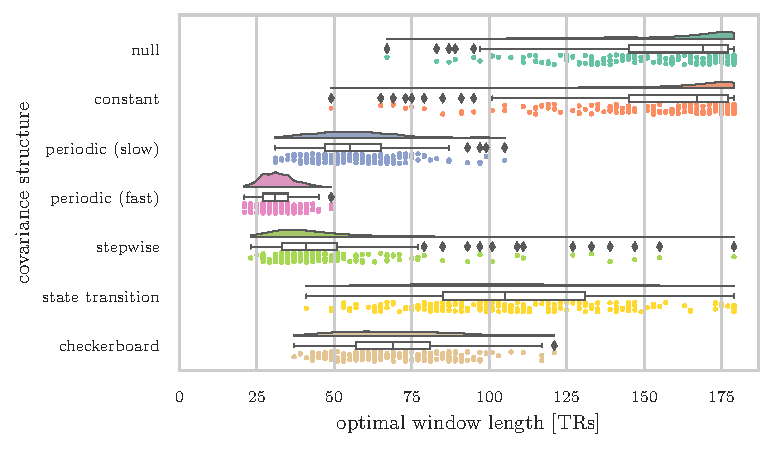
\includegraphics[width=\textwidth]{fig/sim/d2/N1200_T0200/no_noise/SW_cross_validated_optimal_window_lengths}
  \caption{
    Simulations benchmark optimal cross-validated window lengths learned from bivariate ($D = 2$) noiseless data for $N = 1200$.
    Each dot represents one of $T = 200$ trials.
  }\label{fig:sim-optimal-window-lengths-N1200}
\end{figure}


%%
\clearpage
\section{Simulations: Learned kernel lengthscales}\label{appendix:sim-kernel-lengthscales}
%%


\begin{figure}[ht]
    \centering
    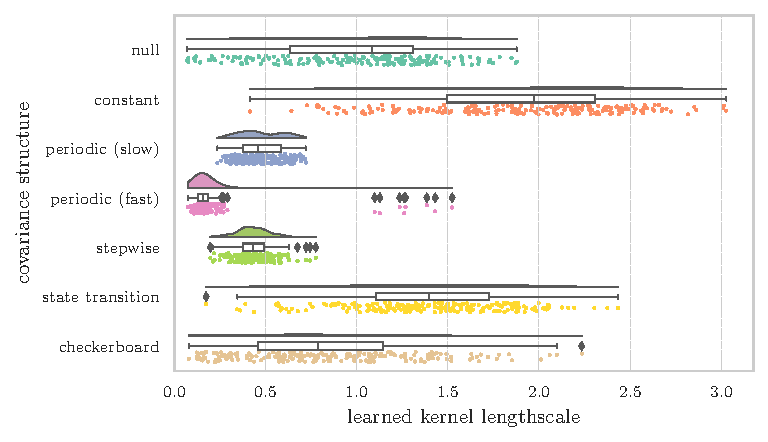
\includegraphics[width=\textwidth]{fig/sim/d2/N0120_T0200/no_noise/SVWP_kernel_lengthscales}
    \caption{
        Simulations benchmark SVWP kernel lengthscales $l$ learned from bivariate ($D = 2$) noiseless data for $N = 120$.
        Each dot represents one of $T = 200$ trials.
    }\label{fig:sim-learned-kernel-lengthscales-N120}
\end{figure}


\begin{figure}[ht]
    \centering
    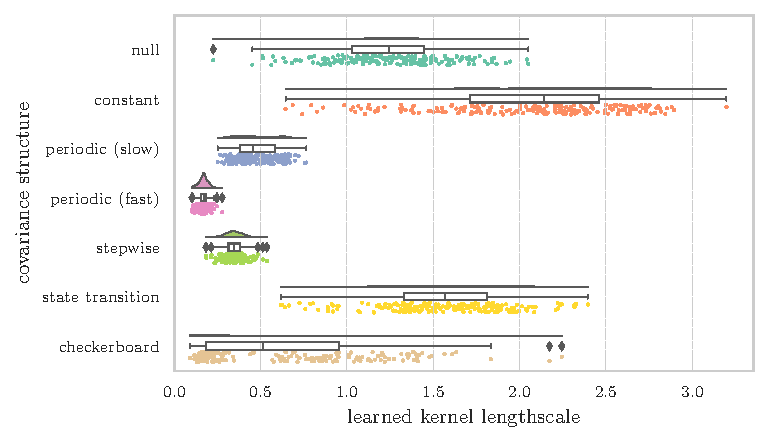
\includegraphics[width=\textwidth]{fig/sim/d2/N0200_T0200/no_noise/SVWP_kernel_lengthscales}
    \caption{
        Simulations benchmark SVWP kernel lengthscales $l$ learned from bivariate ($D = 2$) noiseless data for $N = 200$.
        Each dot represents one of $T = 200$ trials.
    }\label{fig:sim-learned-kernel-lengthscales-N200}
\end{figure}


\begin{figure}[ht]
  \centering
  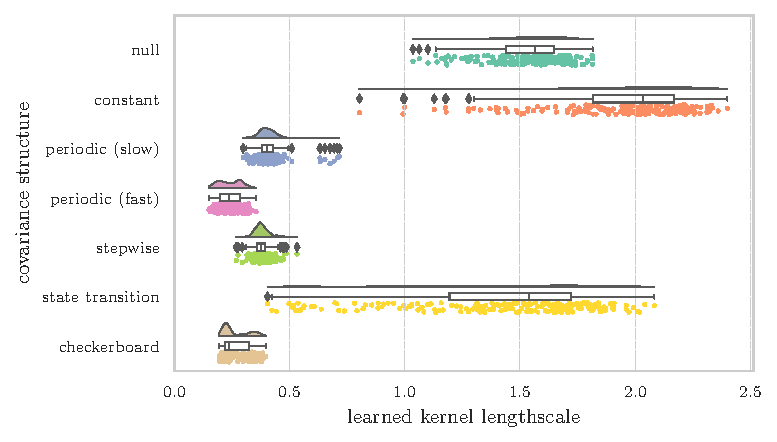
\includegraphics[width=\textwidth]{fig/sim/d2/N1200_T0200/no_noise/SVWP_kernel_lengthscales}
  \caption{
    Simulations benchmark SVWP kernel lengthscales $l$ learned from bivariate ($D = 2$) noiseless data for $N = 1200$.
    Each dot represents one of $T = 200$ trials.
  }\label{fig:sim-learned-kernel-lengthscales-N1200}
\end{figure}


%%
\clearpage
\section{Simulations: Impact of noise}\label{ch:appendix-impact-of-noise}
%%

%%
\subsection{Bivariate TVFC estimates}\label{ch:appendix-d2-impact-of-noise}
%%


\begin{figure}[h]
  \centering
  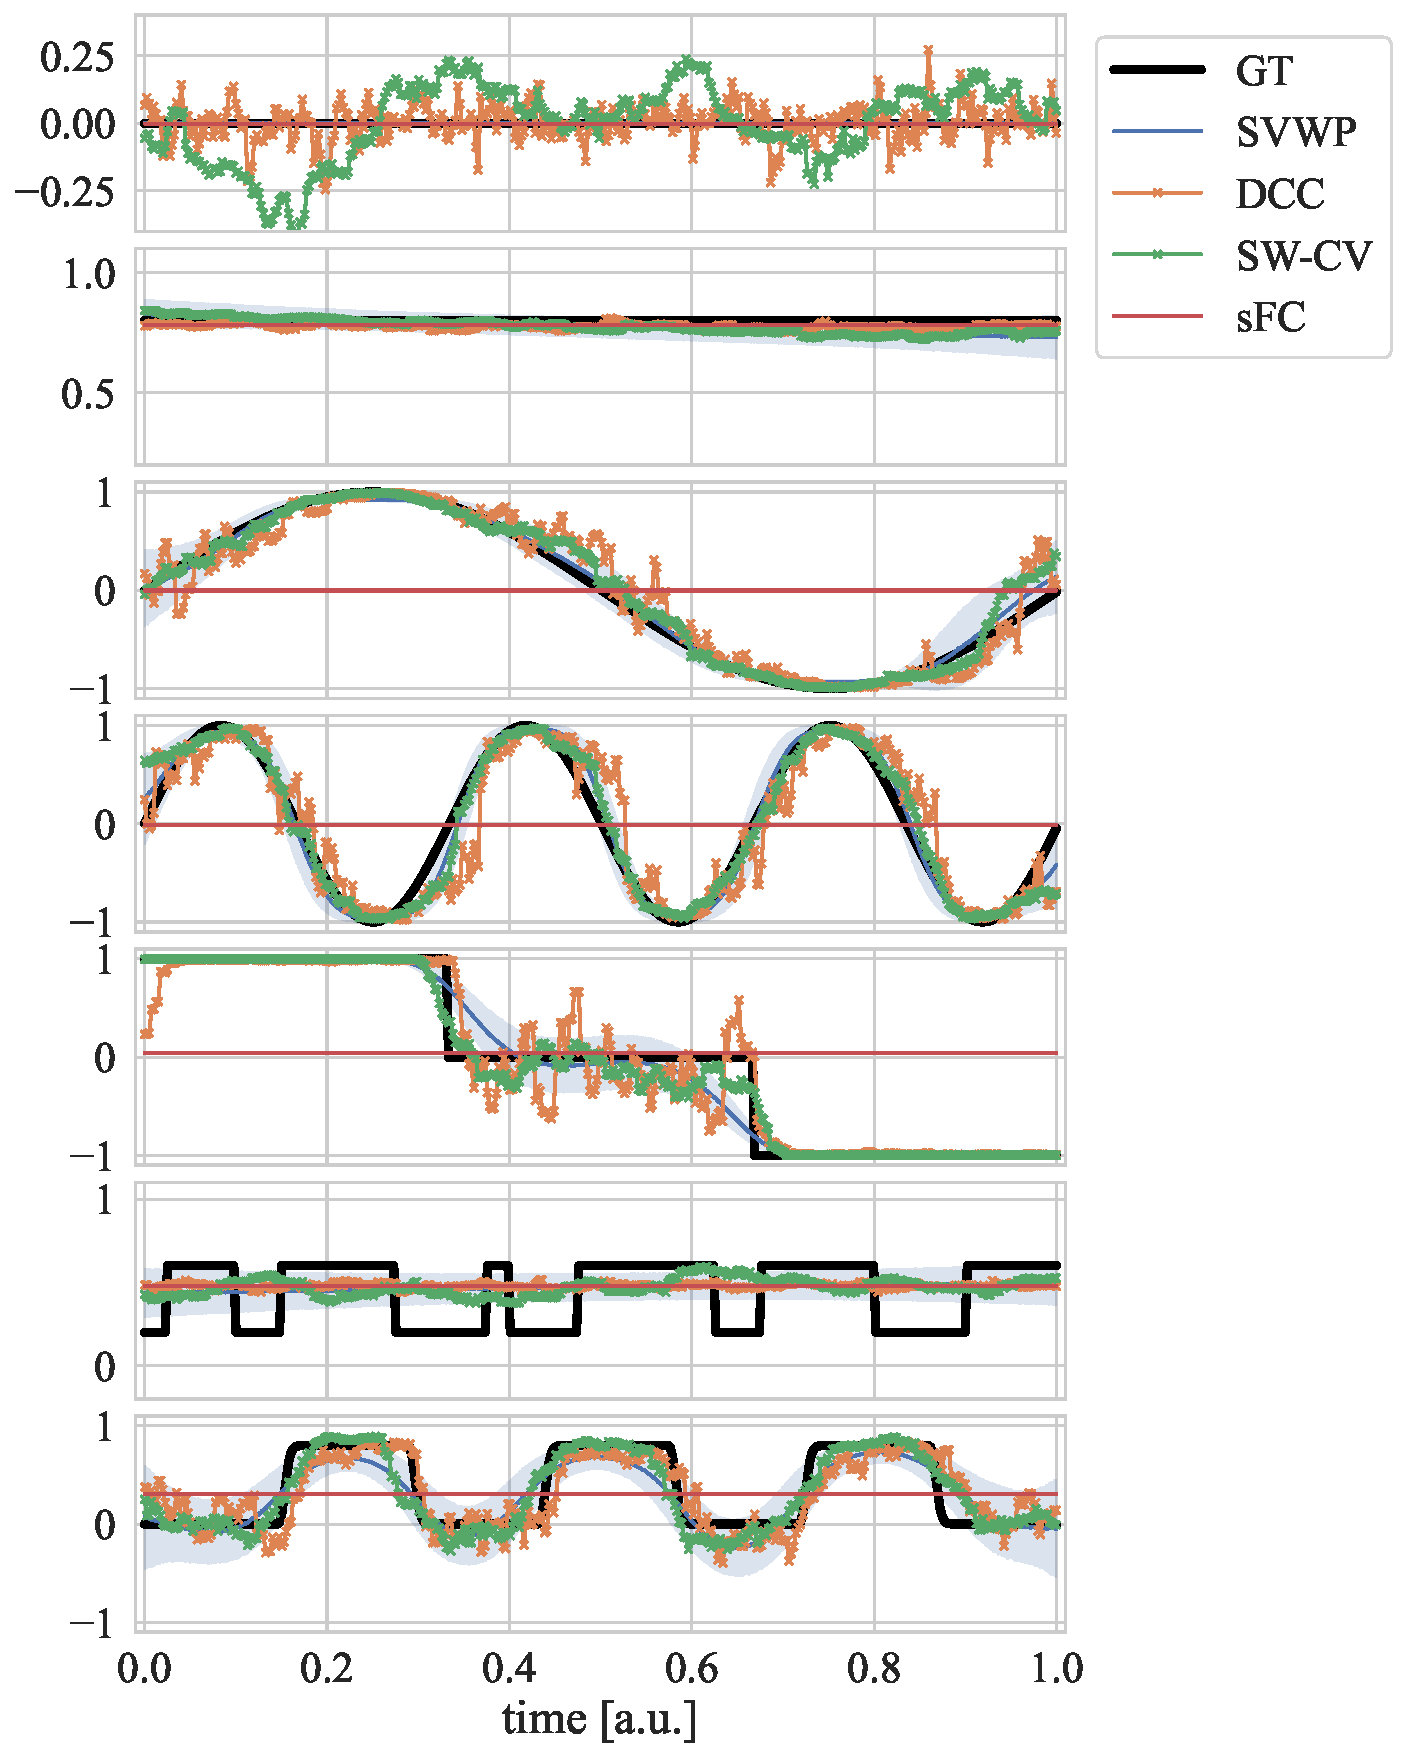
\includegraphics[width=\textwidth]{fig/sim/d2/N0400_T0200/no_noise/all_covs_types_correlations}
  \caption{
    Model TVFC predictions on bivariate data for $N = 400$ data points.
    No noise added.
  }\label{fig:results-all-covariance-structures-tvfc-predictions}
\end{figure}


\begin{figure}[h]
  \centering
  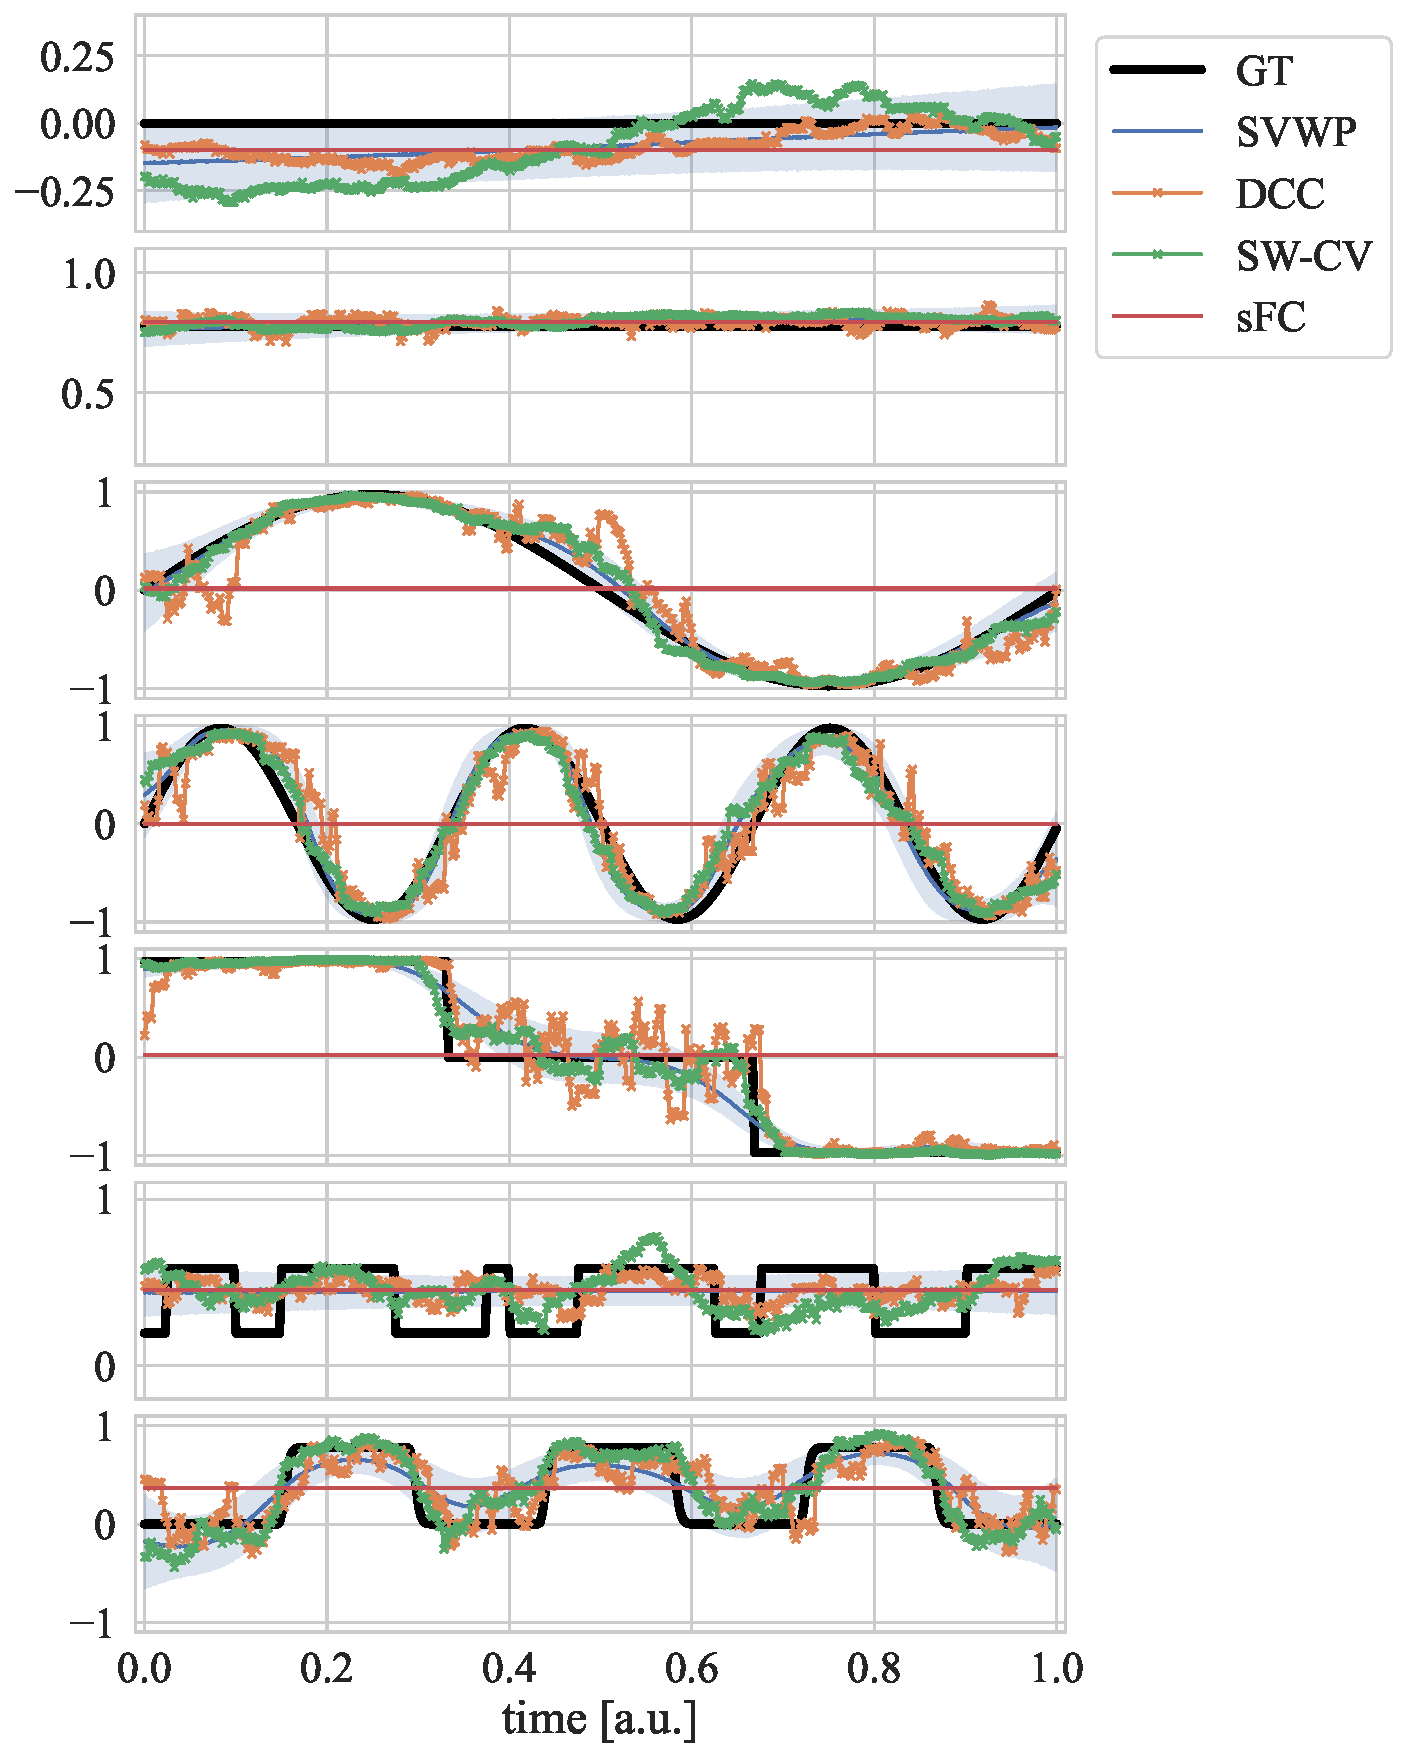
\includegraphics[width=\textwidth]{fig/sim/d2/N0400_T0200/HCP_noise_snr_6/all_covs_types_correlations}
  \caption{
    Model TVFC predictions on bivariate data for $N=400$ data points.
    HCP noise with SNR of 6 added.
  }\label{fig:results-all-covariance-structures-tvfc-predictions-snr-6}
\end{figure}


\begin{figure}[h]
  \centering
  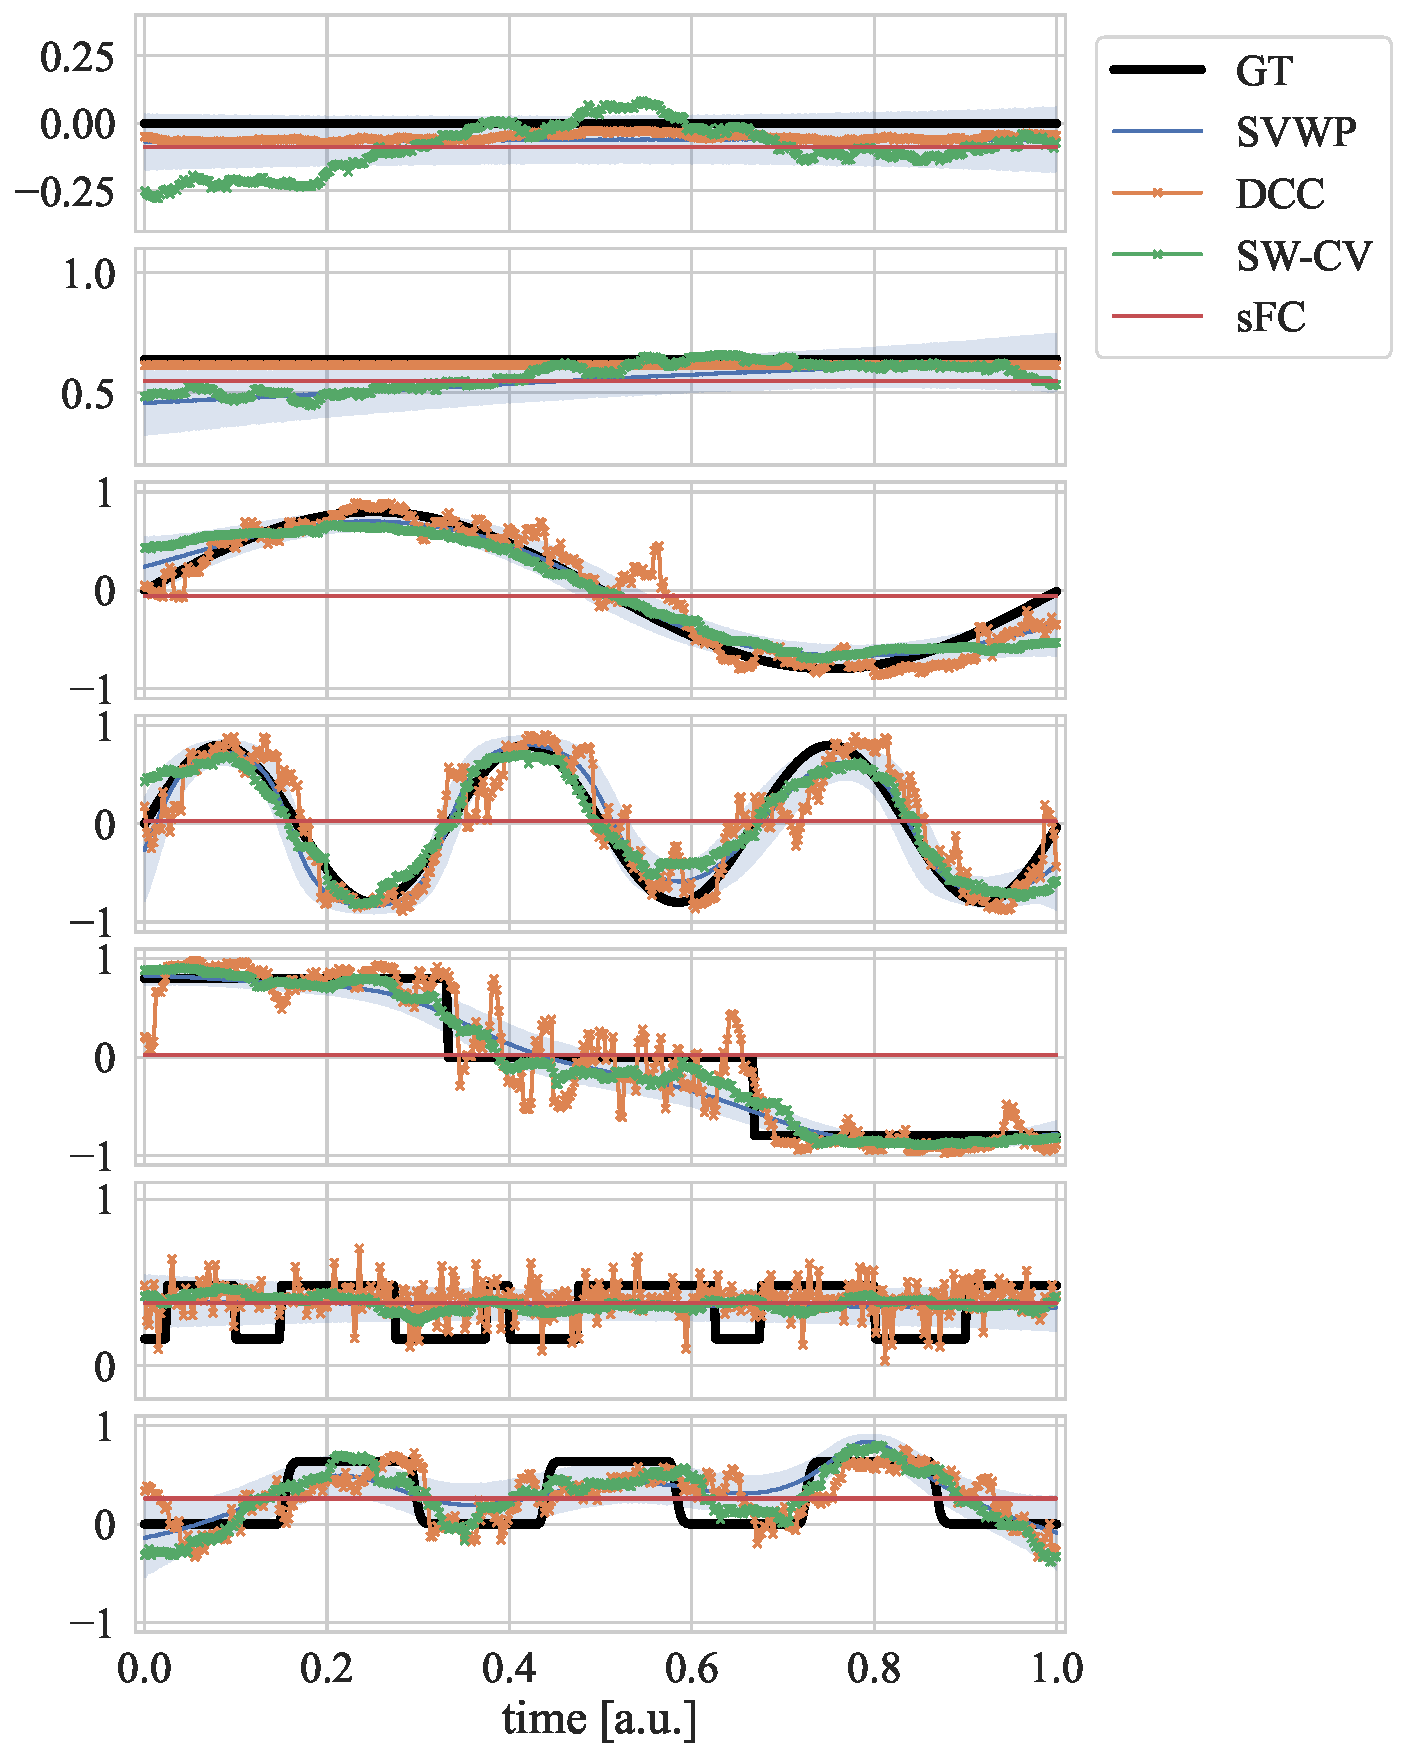
\includegraphics[width=\textwidth]{fig/sim/d2/N0400_T0200/HCP_noise_snr_2/all_covs_types_correlations}
  \caption{
    Model TVFC predictions on bivariate data for $N = 400$ data points.
    HCP noise with SNR of 2 added.
  }\label{fig:results-all-covariance-structures-tvfc-predictions-snr-2}
\end{figure}


\begin{figure}[h]
  \centering
  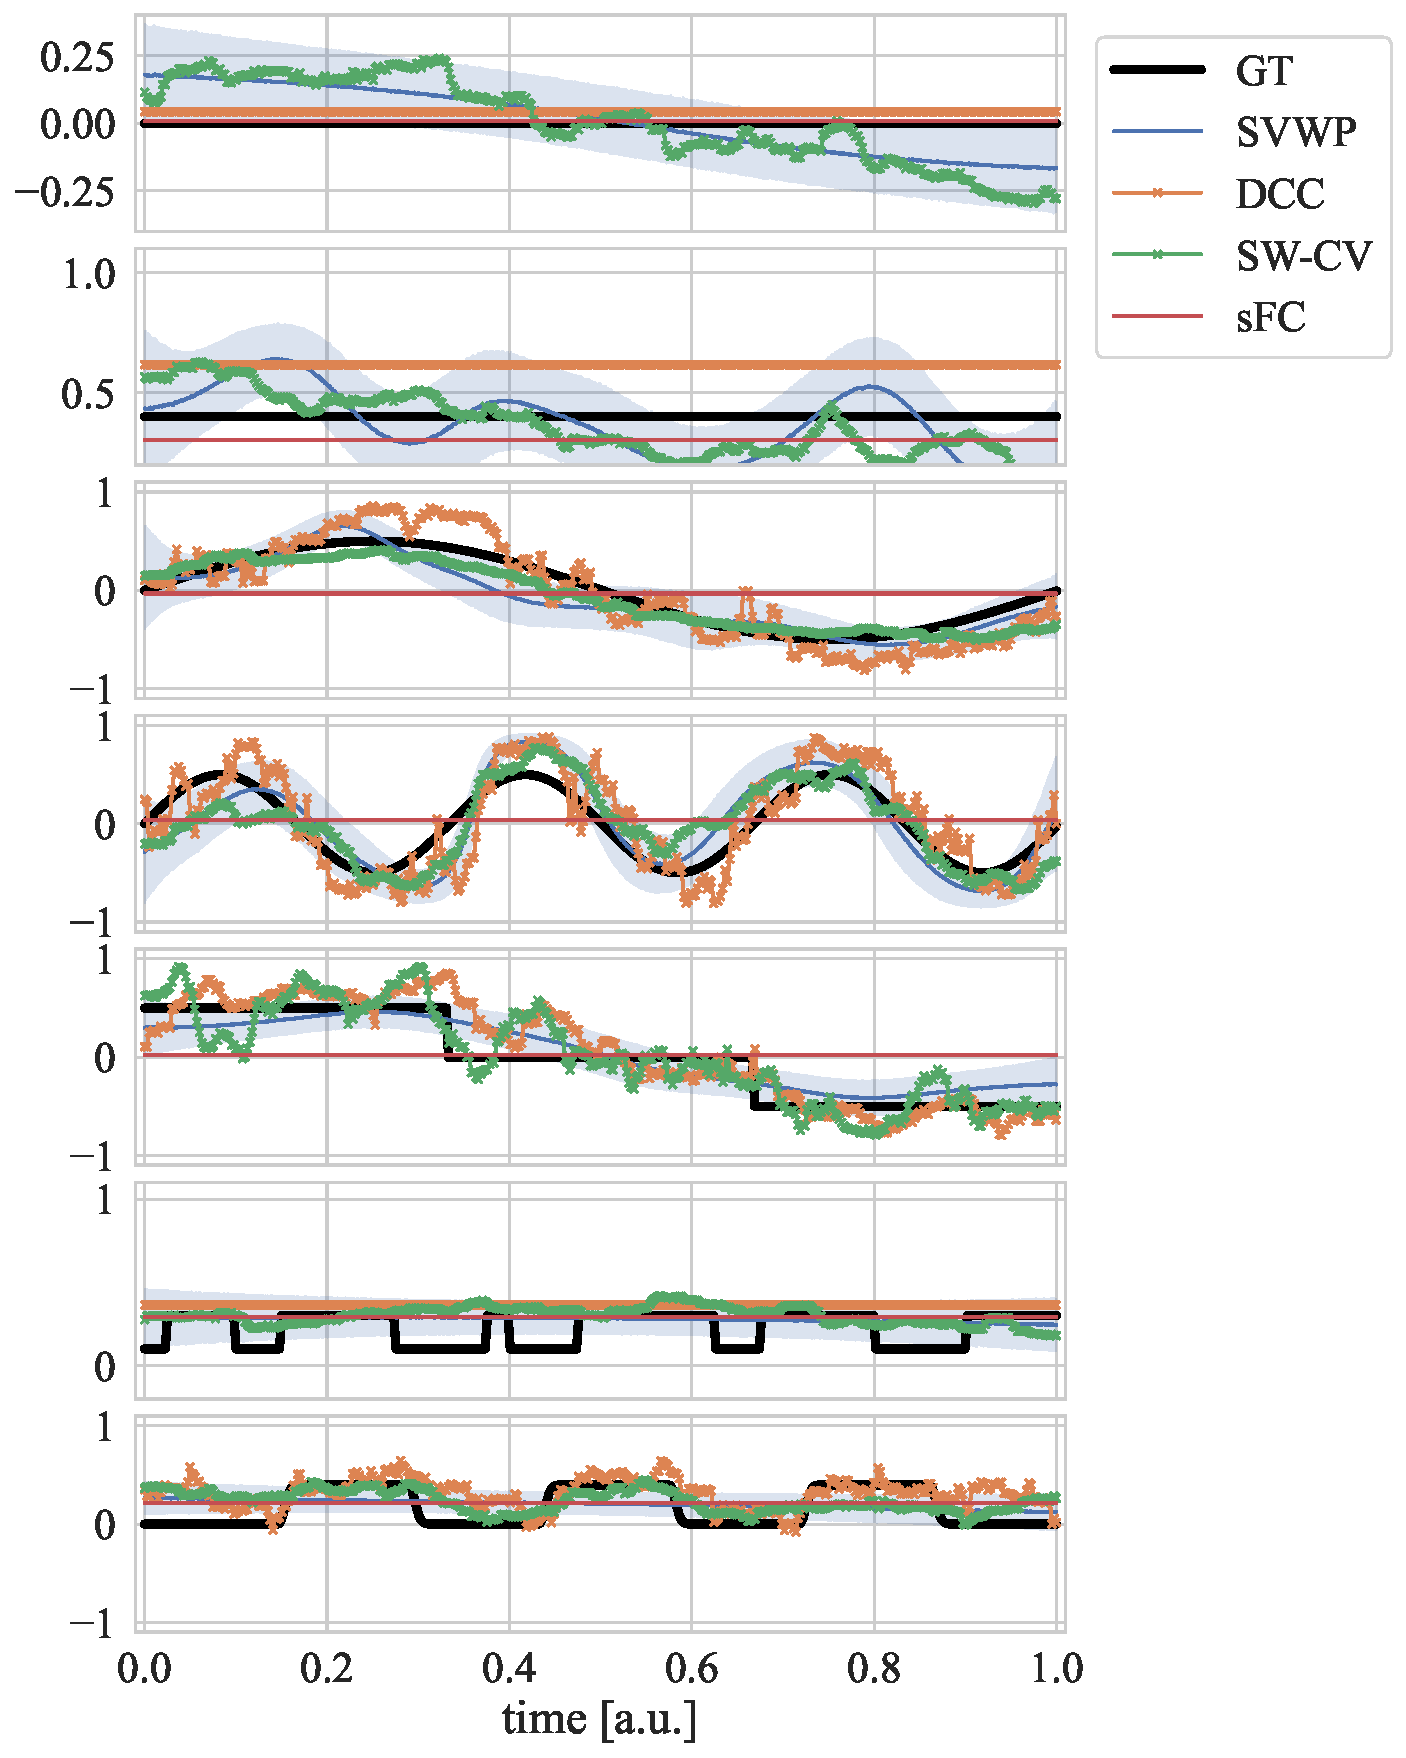
\includegraphics[width=\textwidth]{fig/sim/d2/N0400_T0200/HCP_noise_snr_1/all_covs_types_correlations}
  \caption{
    Model TVFC predictions on bivariate data for $N = 400$ data points.
    HCP noise with SNR of 1 added.
  }\label{fig:results-all-covariance-structures-tvfc-predictions-snr-1}
\end{figure}


%%
\clearpage
\subsection{Bivariate quantitative results}
%%


\begin{figure}[ht]
  \centering
  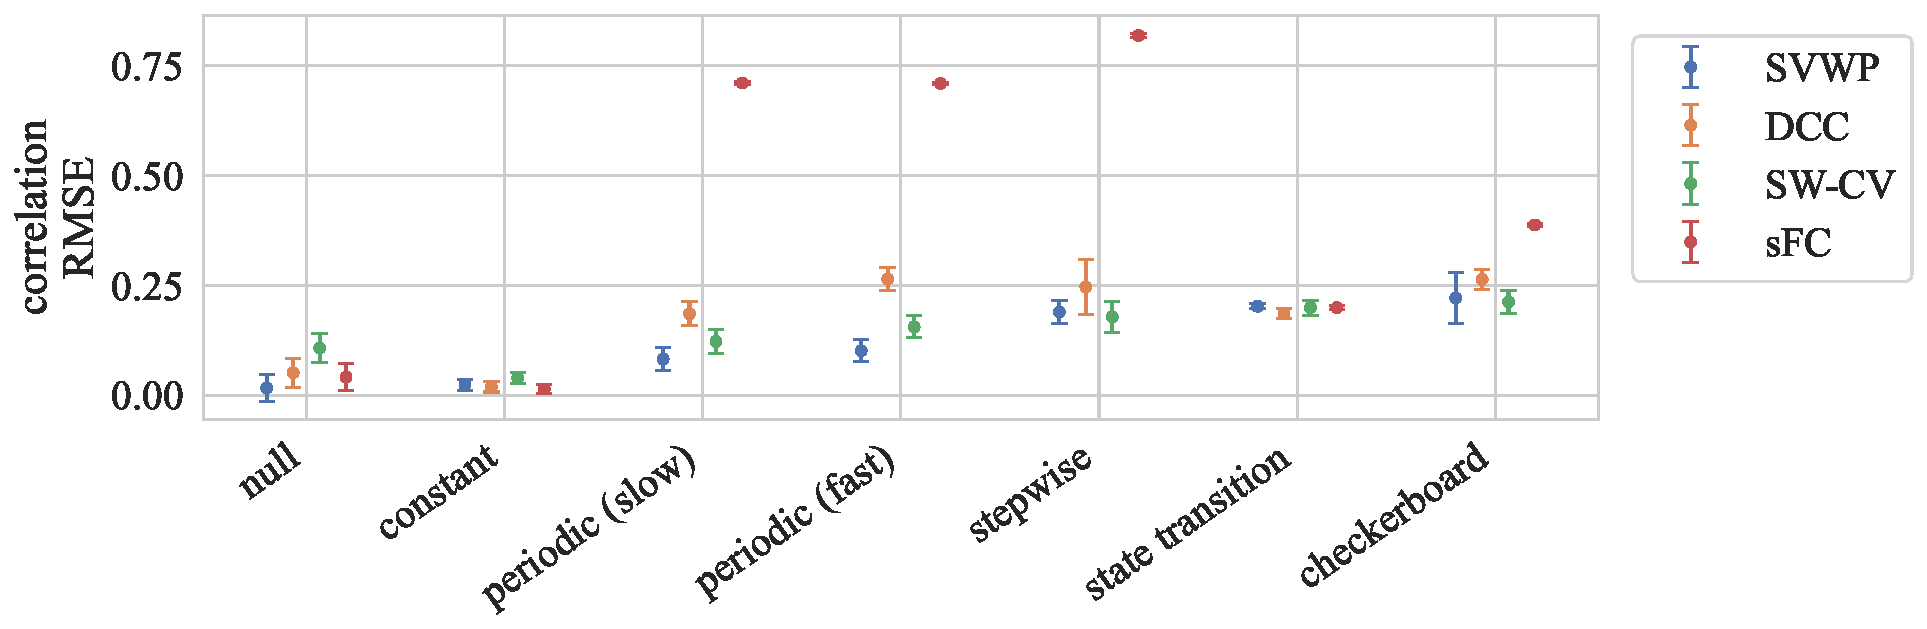
\includegraphics[width=0.84\textwidth]{fig/sim/d2/N0400_T0200/no_noise/correlation_RMSE}
  \caption{
    Performance of models on all bivariate synthetic covariance structures without noise for $N = 400$.
    Means and standard deviations are shown across $T = 200$ trials.
  }\label{fig:results-sim-d2-400-all-correlation-RMSE-no-noise}
\end{figure}


\begin{figure}[ht]
  \centering
  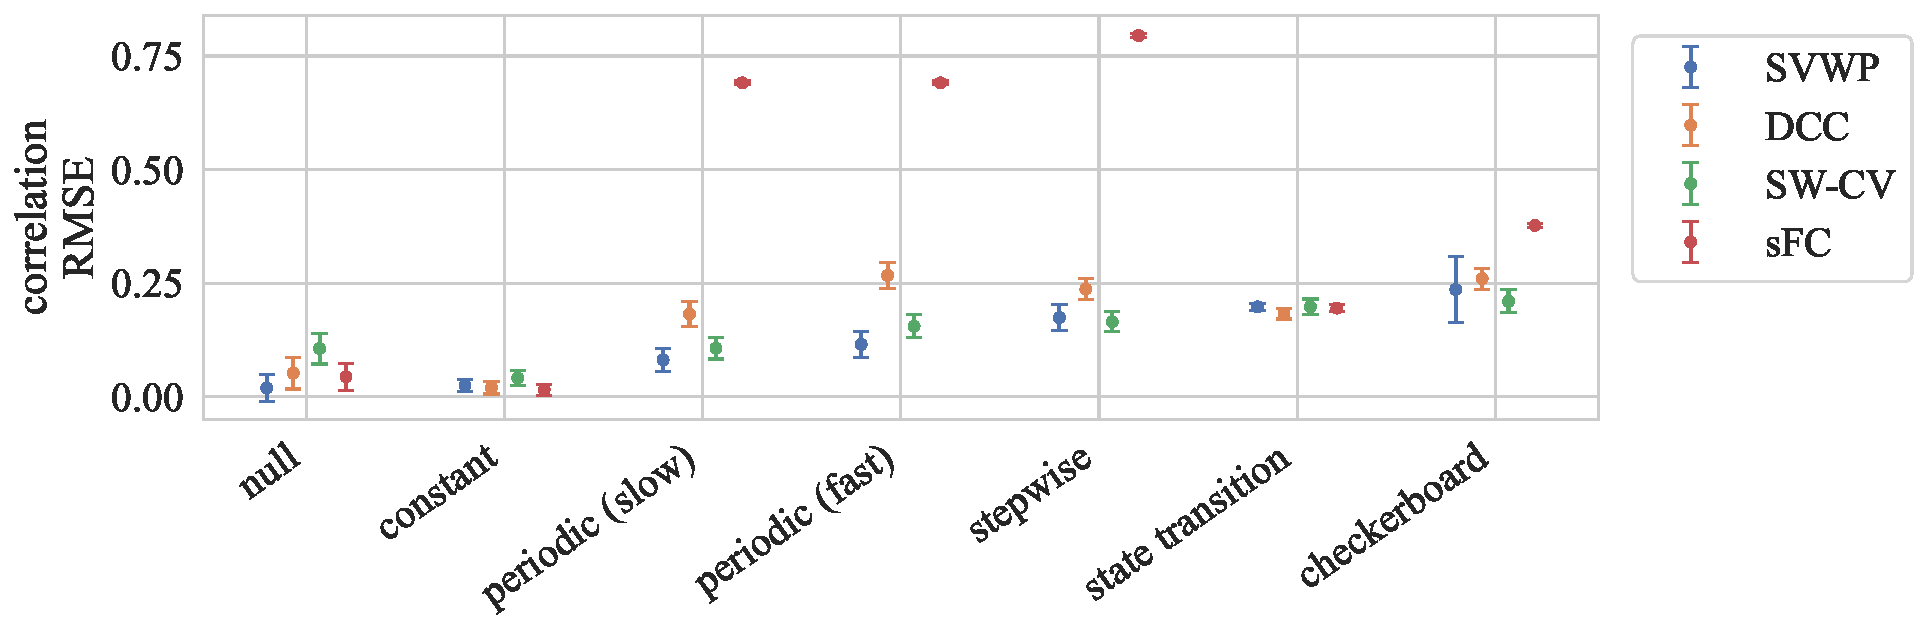
\includegraphics[width=0.84\textwidth]{fig/sim/d2/N0400_T0200/HCP_noise_snr_6/correlation_RMSE}
  \caption{
    Performance of models on all bivariate synthetic covariance structures with HCP noise with SNR of 6 added for $N = 400$.
    Means and standard deviations are shown across $T = 200$ trials.
  }\label{fig:results-sim-d2-400-all-correlation-RMSE-snr-6}
\end{figure}


\begin{figure}[ht]
  \centering
  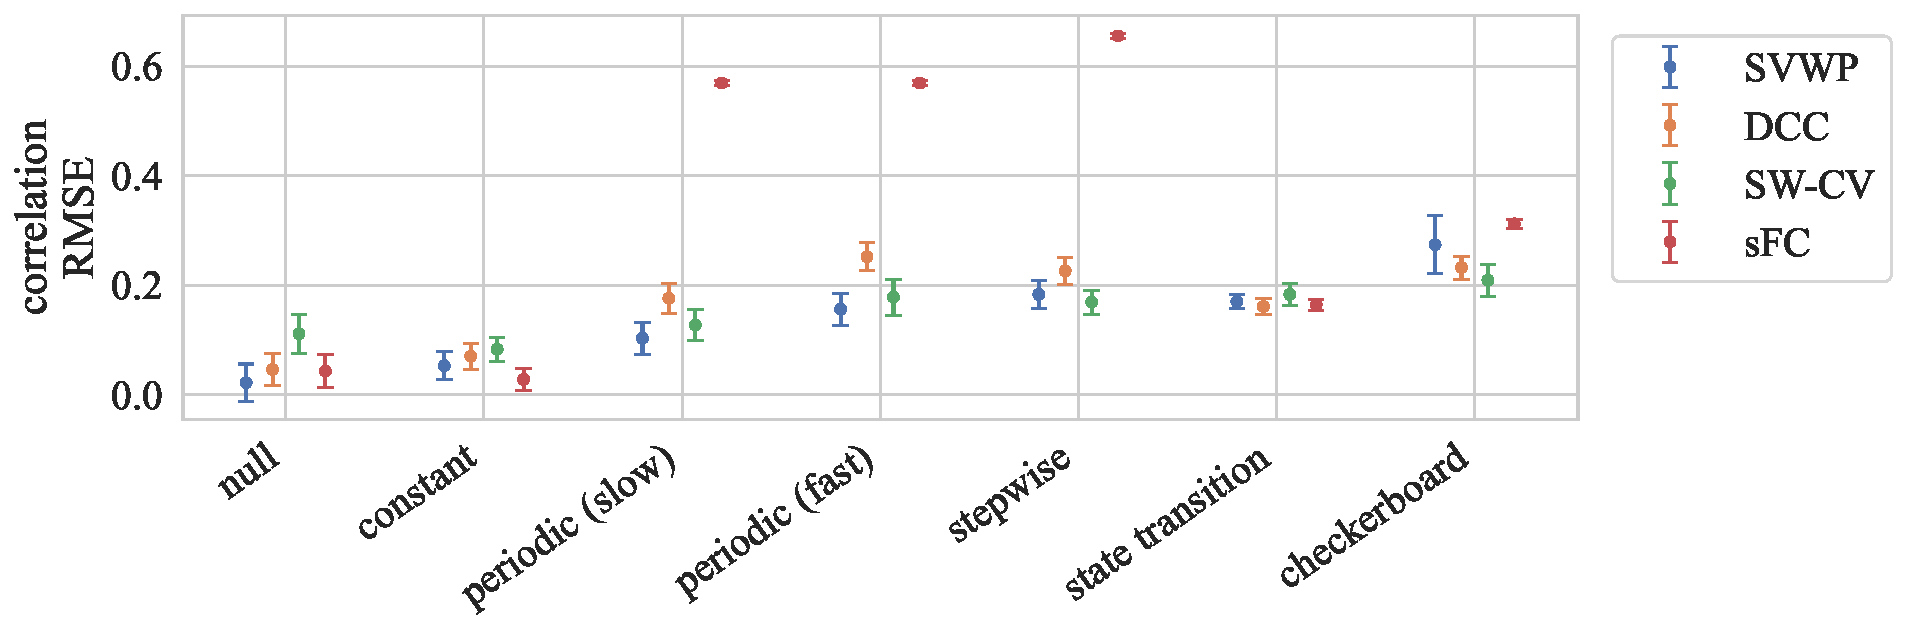
\includegraphics[width=0.84\textwidth]{fig/sim/d2/N0400_T0200/HCP_noise_snr_2/correlation_RMSE}
  \caption{
    Performance of models on all bivariate synthetic covariance structures with HCP noise with SNR of 2 added for $N = 400$.
    Means and standard deviations are shown across $T = 200$ trials.
  }\label{fig:results-sim-d2-400-all-correlation-RMSE-snr-2}
\end{figure}


\begin{figure}[ht]
  \centering
  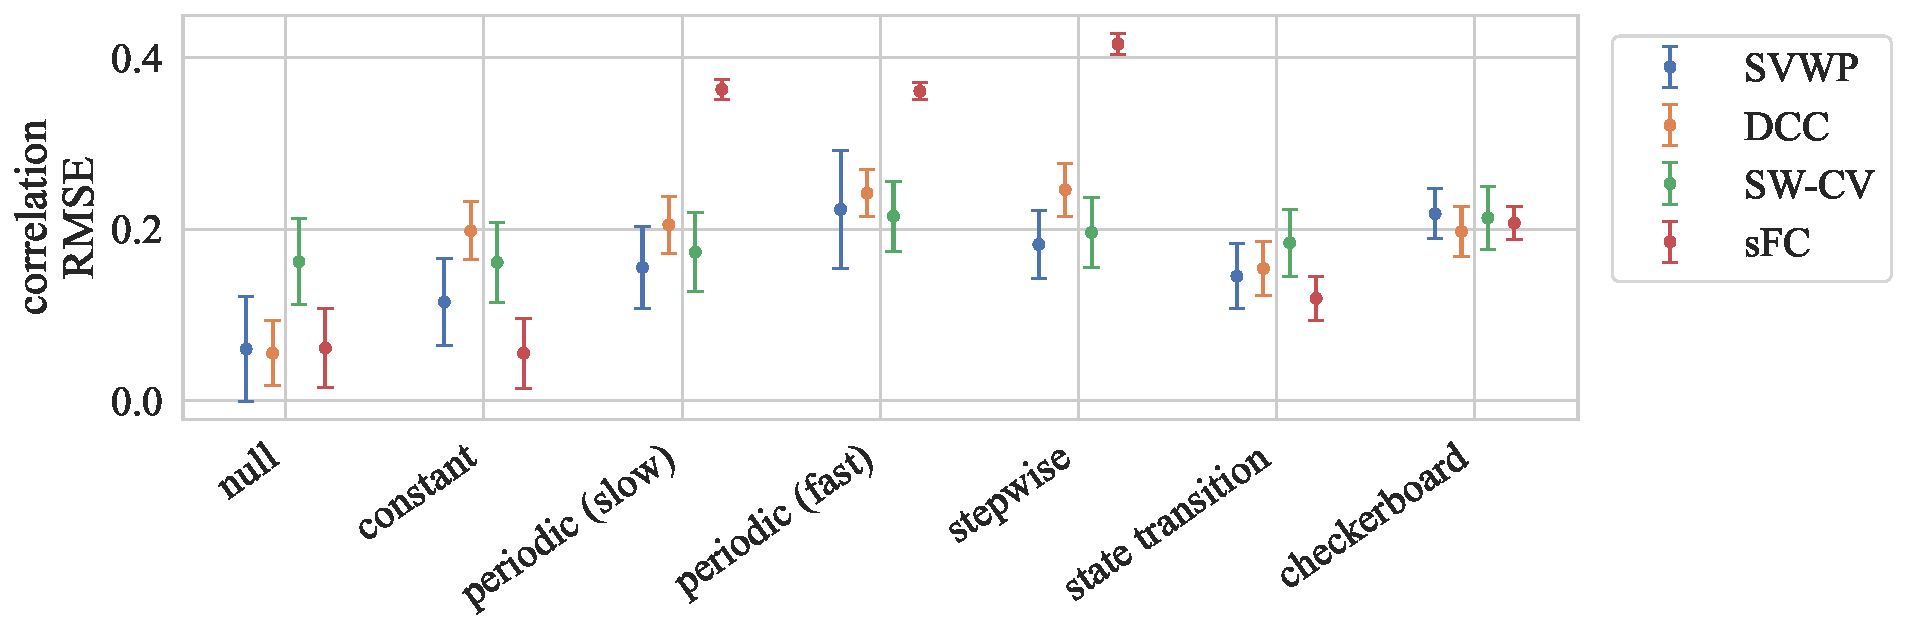
\includegraphics[width=0.84\textwidth]{fig/sim/d2/N0400_T0200/HCP_noise_snr_1/correlation_RMSE}
  \caption{
    Performance of models on all bivariate synthetic covariance structures with HCP noise with SNR of 1 added for $N = 400$.
    Means and standard deviations are shown across $T = 200$ trials.
  }\label{fig:results-sim-d2-400-all-correlation-RMSE-snr-1}
\end{figure}


%%
\clearpage
\subsection{Trivariate TVFC estimates}\label{ch:appendix-d3d-impact-of-noise}
%%


\begin{figure}[h]
    \centering
    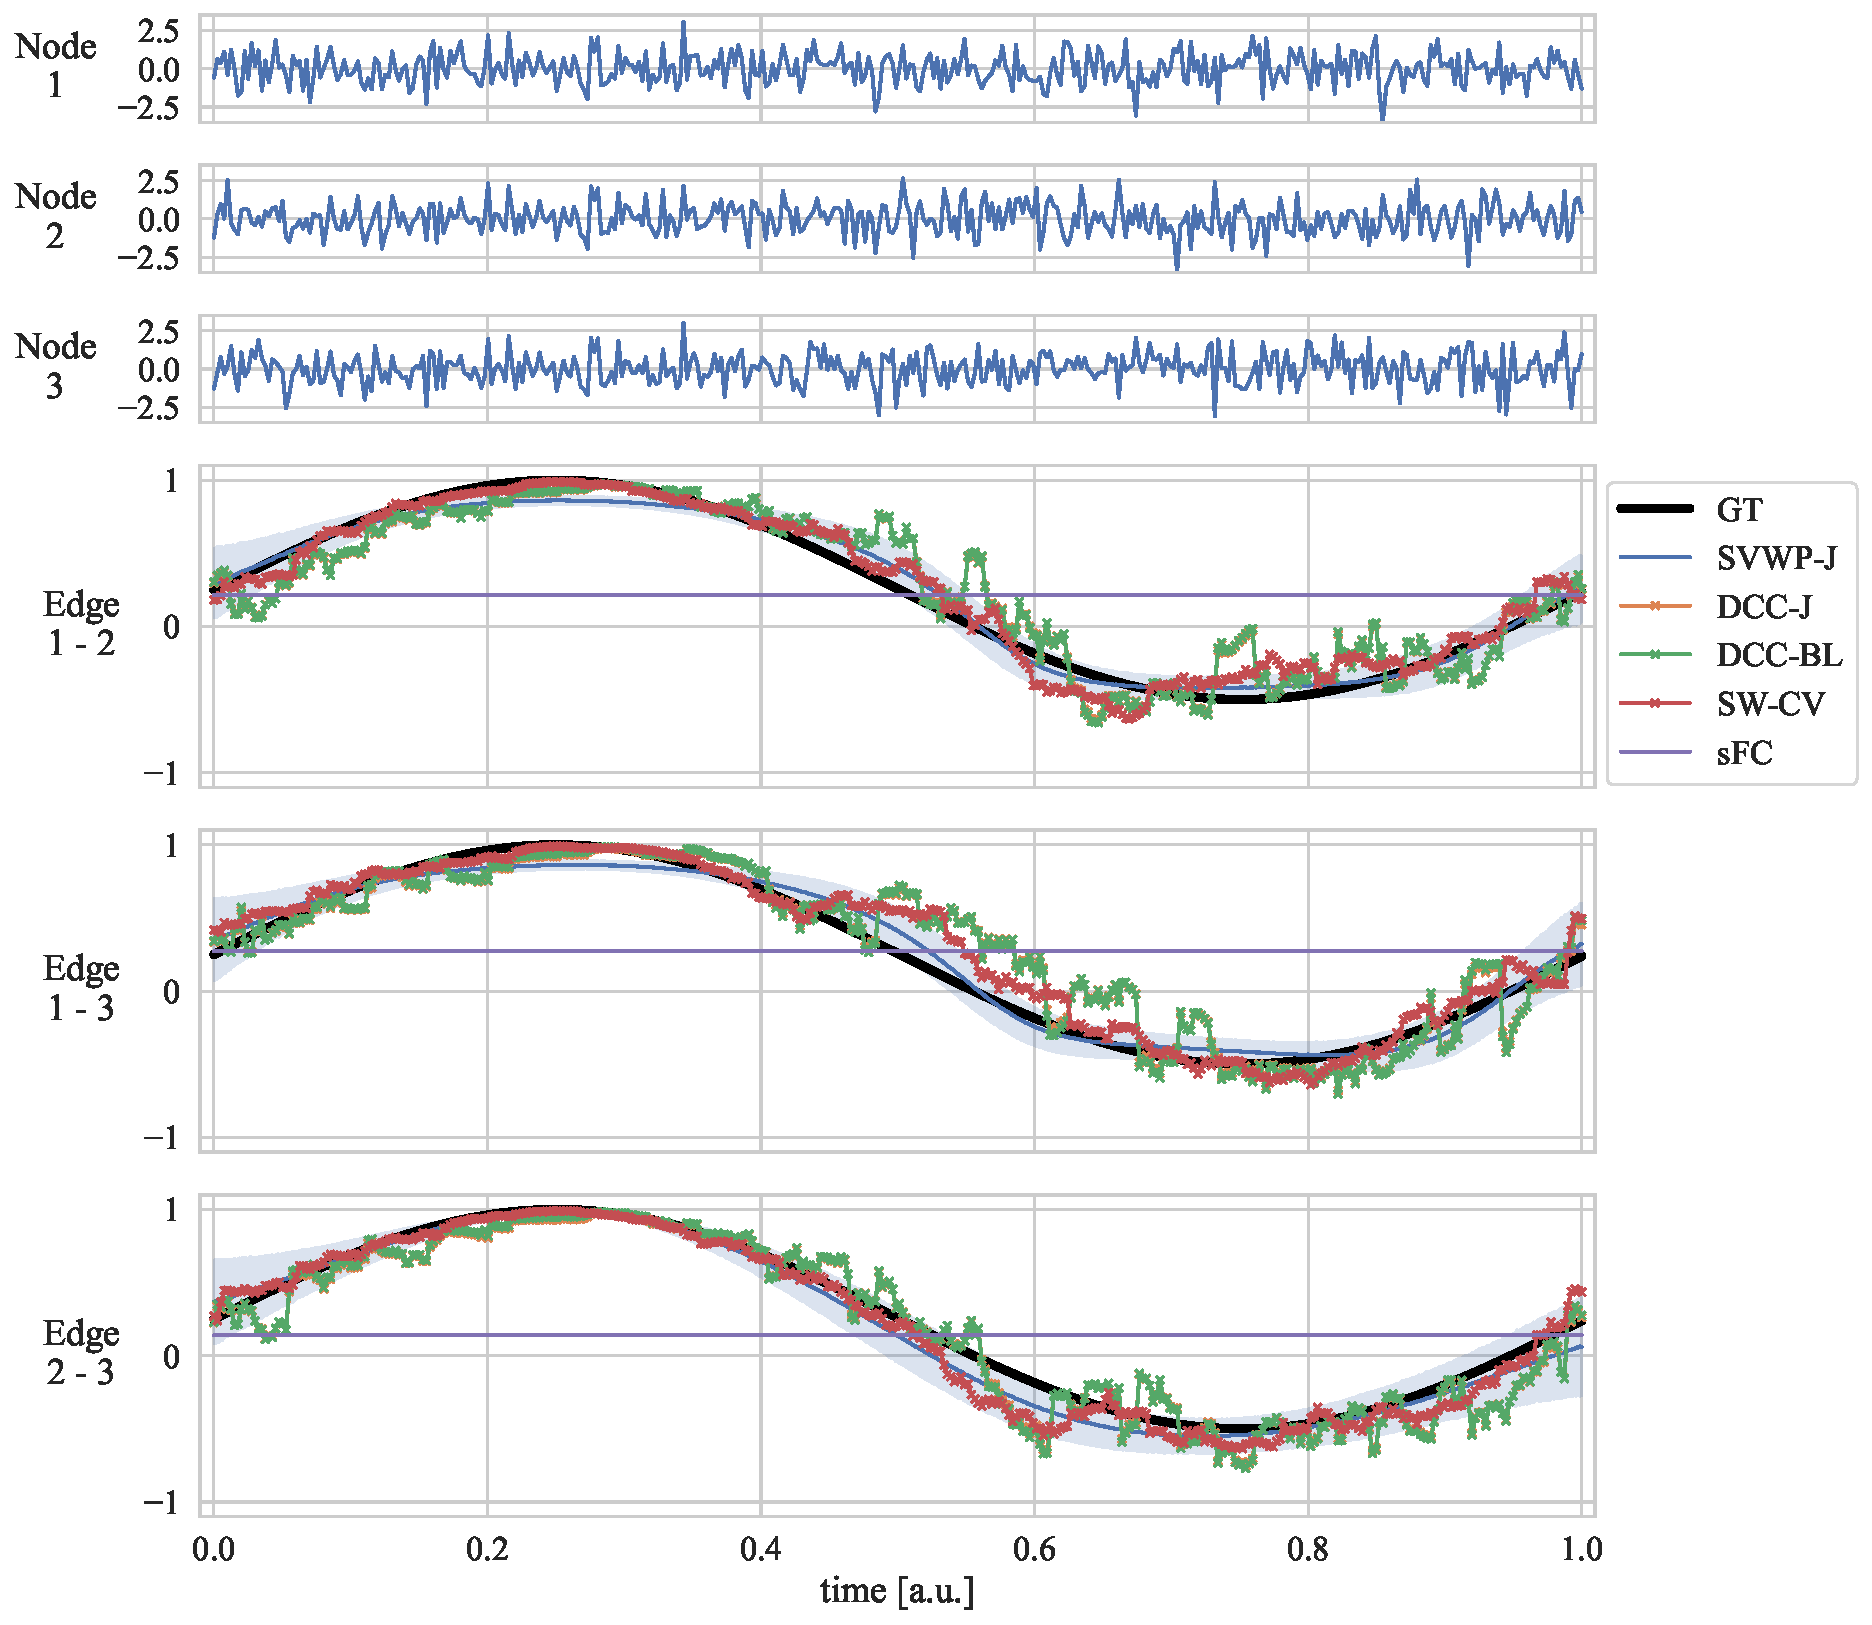
\includegraphics[width=\textwidth]{fig/sim/d3d/N0400_T0003/no_noise/periodic_1_correlations}
    \caption{
        Model TVFC estimates on dense trivariate data for $N = 400$ data points.
        No noise added.
    }\label{fig:results-d3d-periodic-1-tvfc-predictions-no-noise}
\end{figure}


\begin{figure}[h]
    \centering
    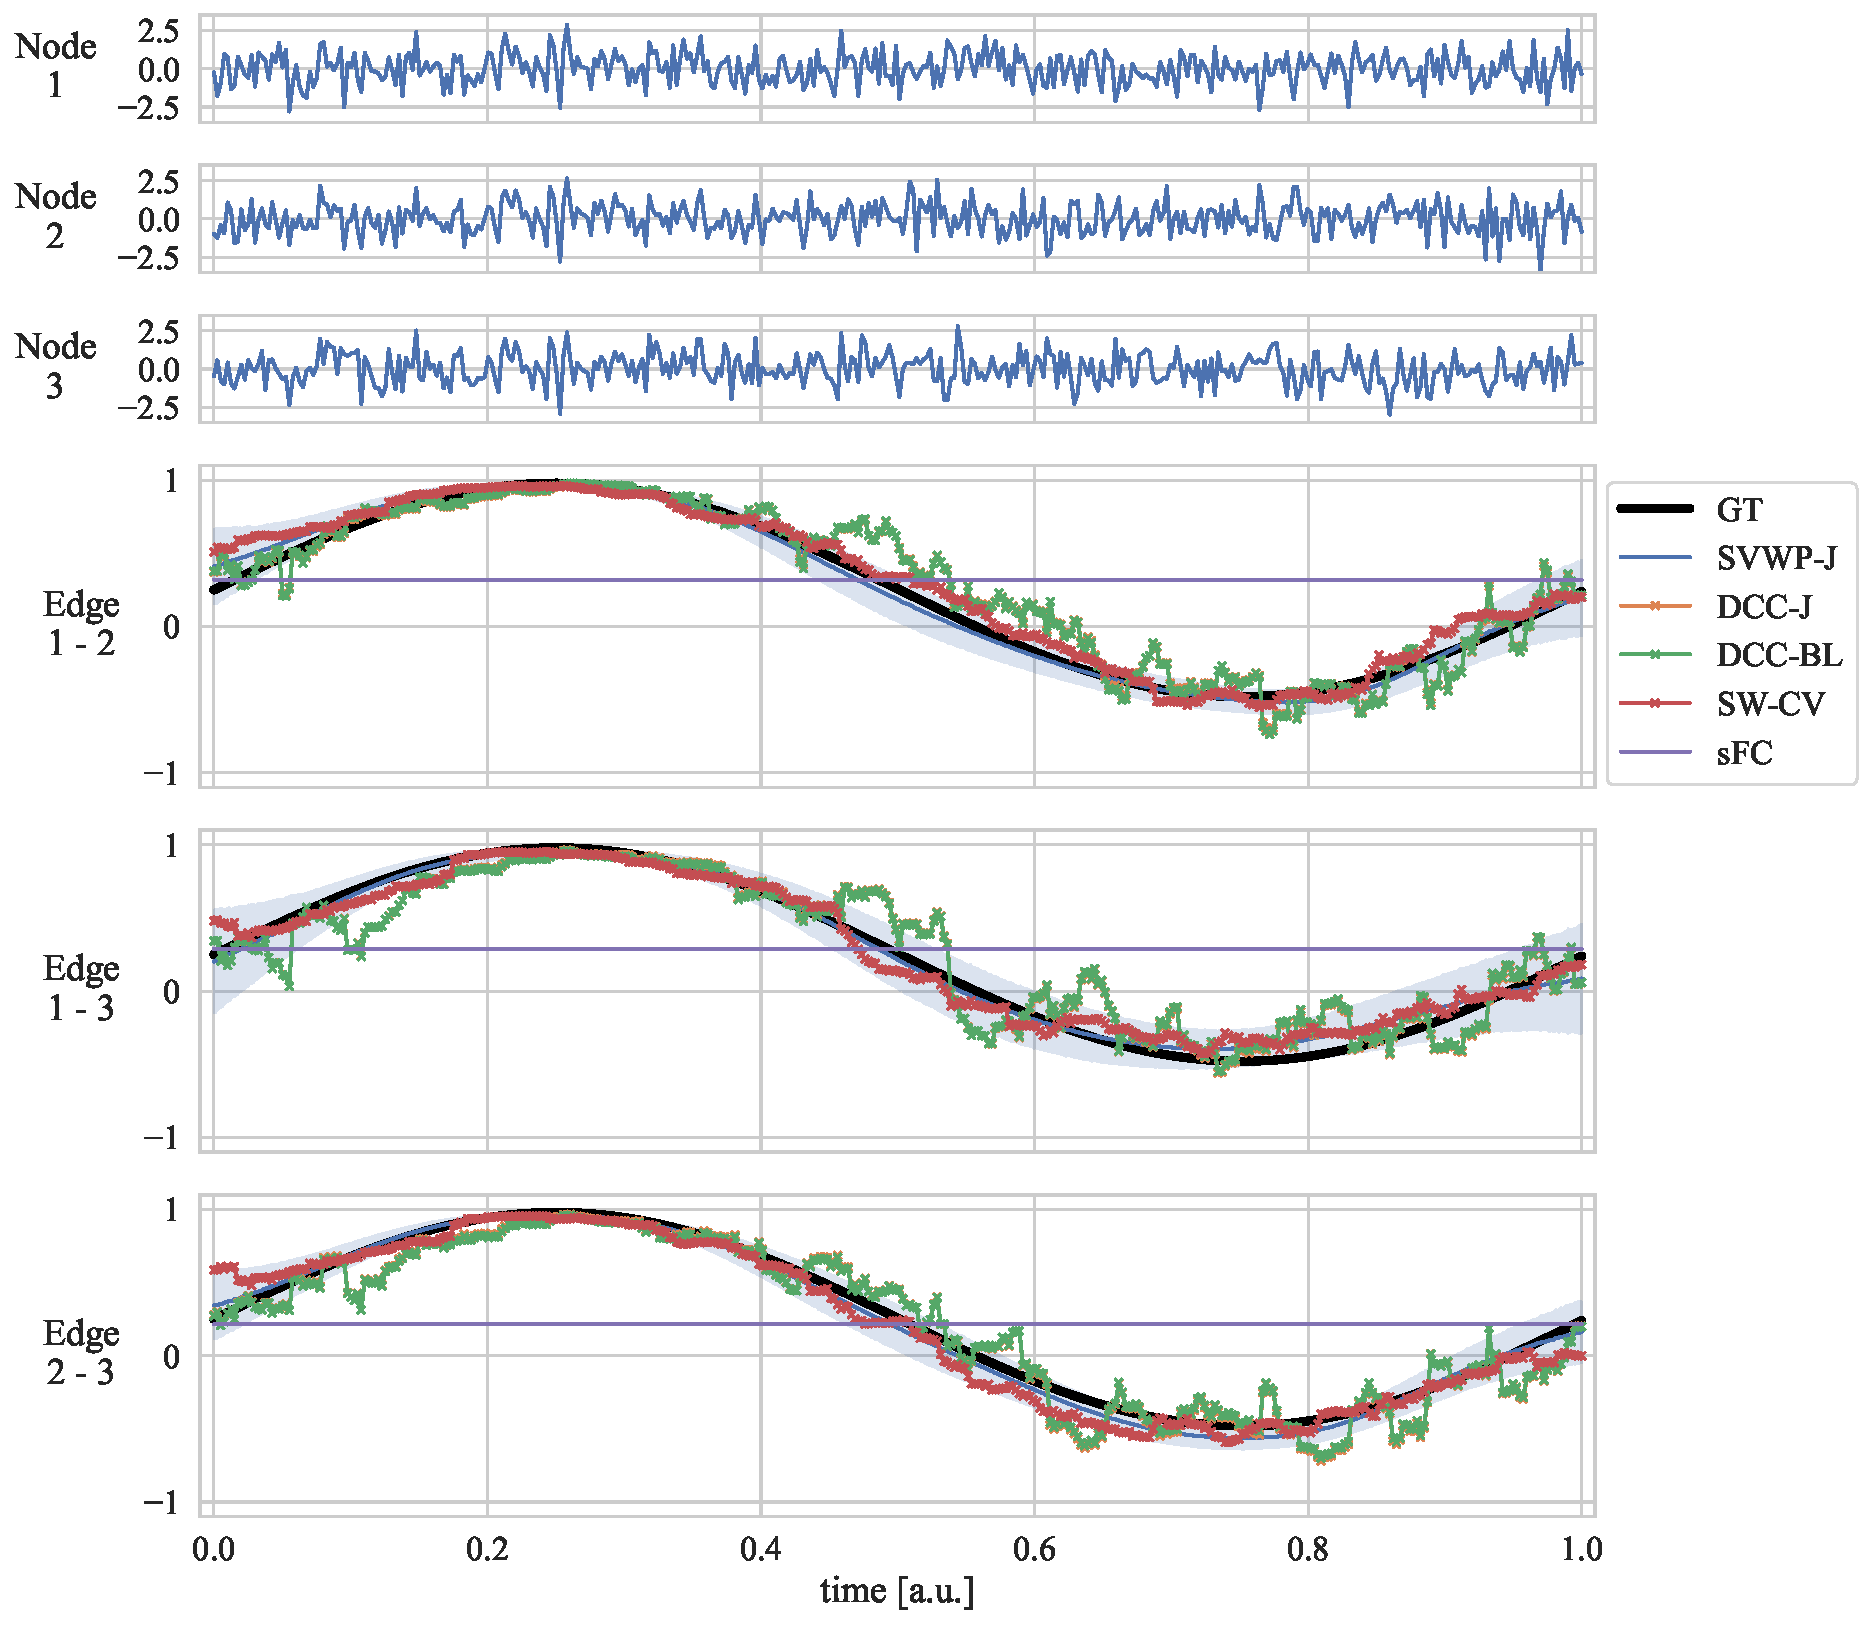
\includegraphics[width=\textwidth]{fig/sim/d3d/N0400_T0003/HCP_noise_snr_6/periodic_1_correlations}
    \caption{
        Model TVFC estimates on dense trivariate data for $N = 400$ data points.
        HCP noise with SNR of 6 added.
    }\label{fig:results-d3d-periodic-1-tvfc-predictions-snr-6}
\end{figure}


\begin{figure}[h]
  \centering
  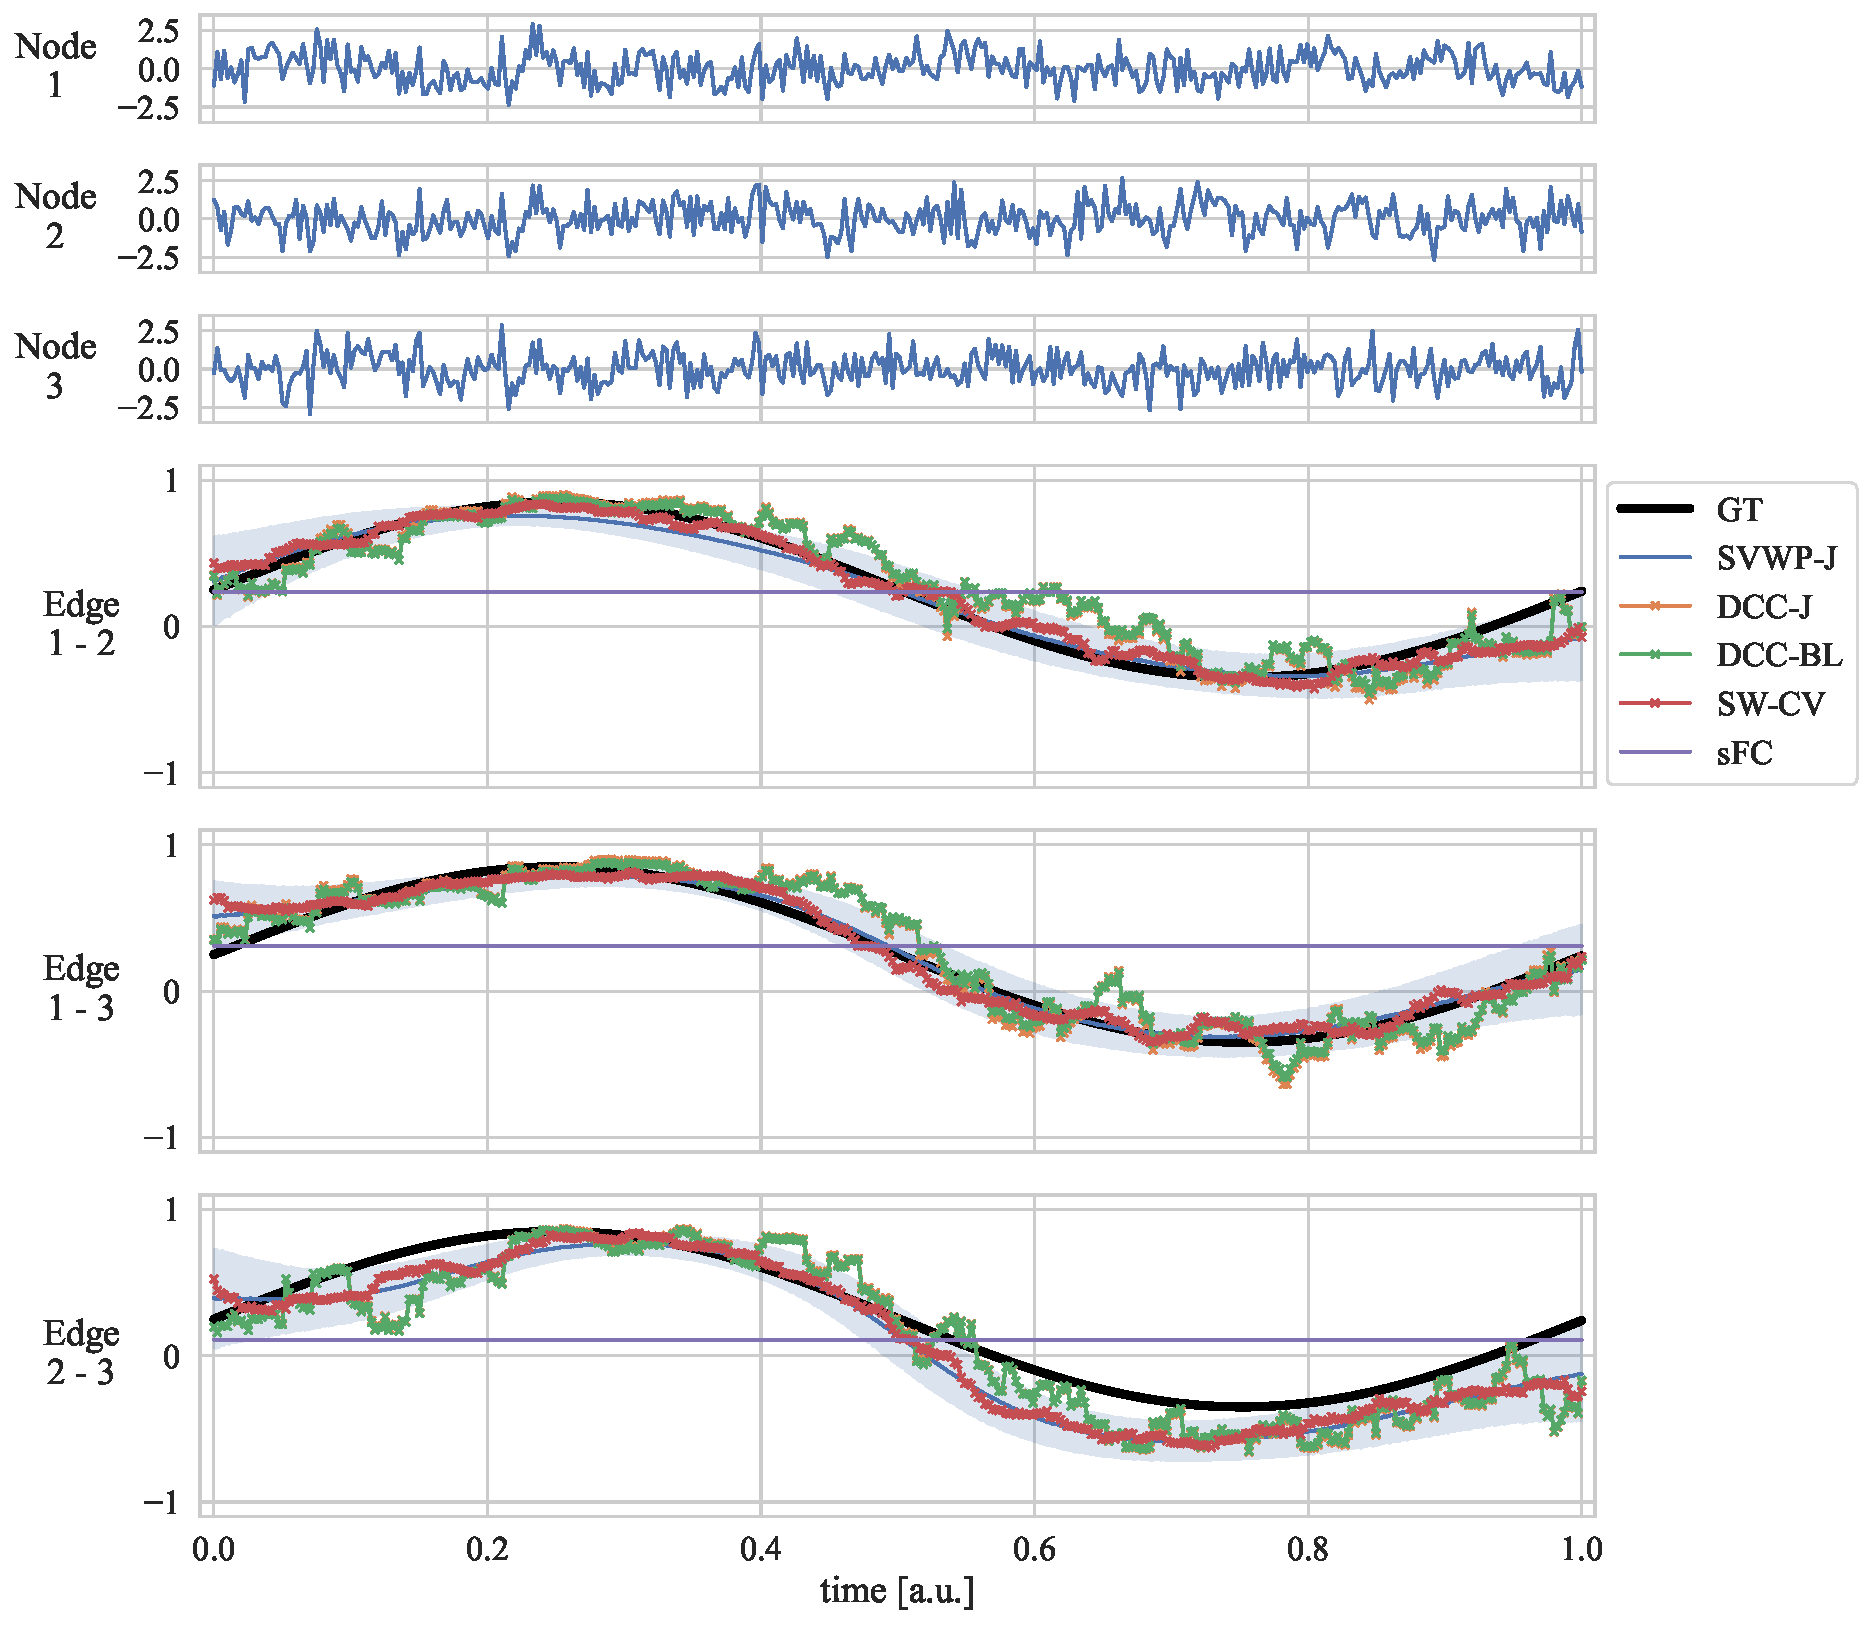
\includegraphics[width=\textwidth]{fig/sim/d3d/N0400_T0003/HCP_noise_snr_2/periodic_1_correlations}
  \caption{
    Model TVFC estimates on dense trivariate data for $N = 400$ data points.
    HCP noise with SNR of 2 added.
  }\label{fig:results-d3d-periodic-1-tvfc-predictions-snr-2}
\end{figure}


\begin{figure}[h]
  \centering
  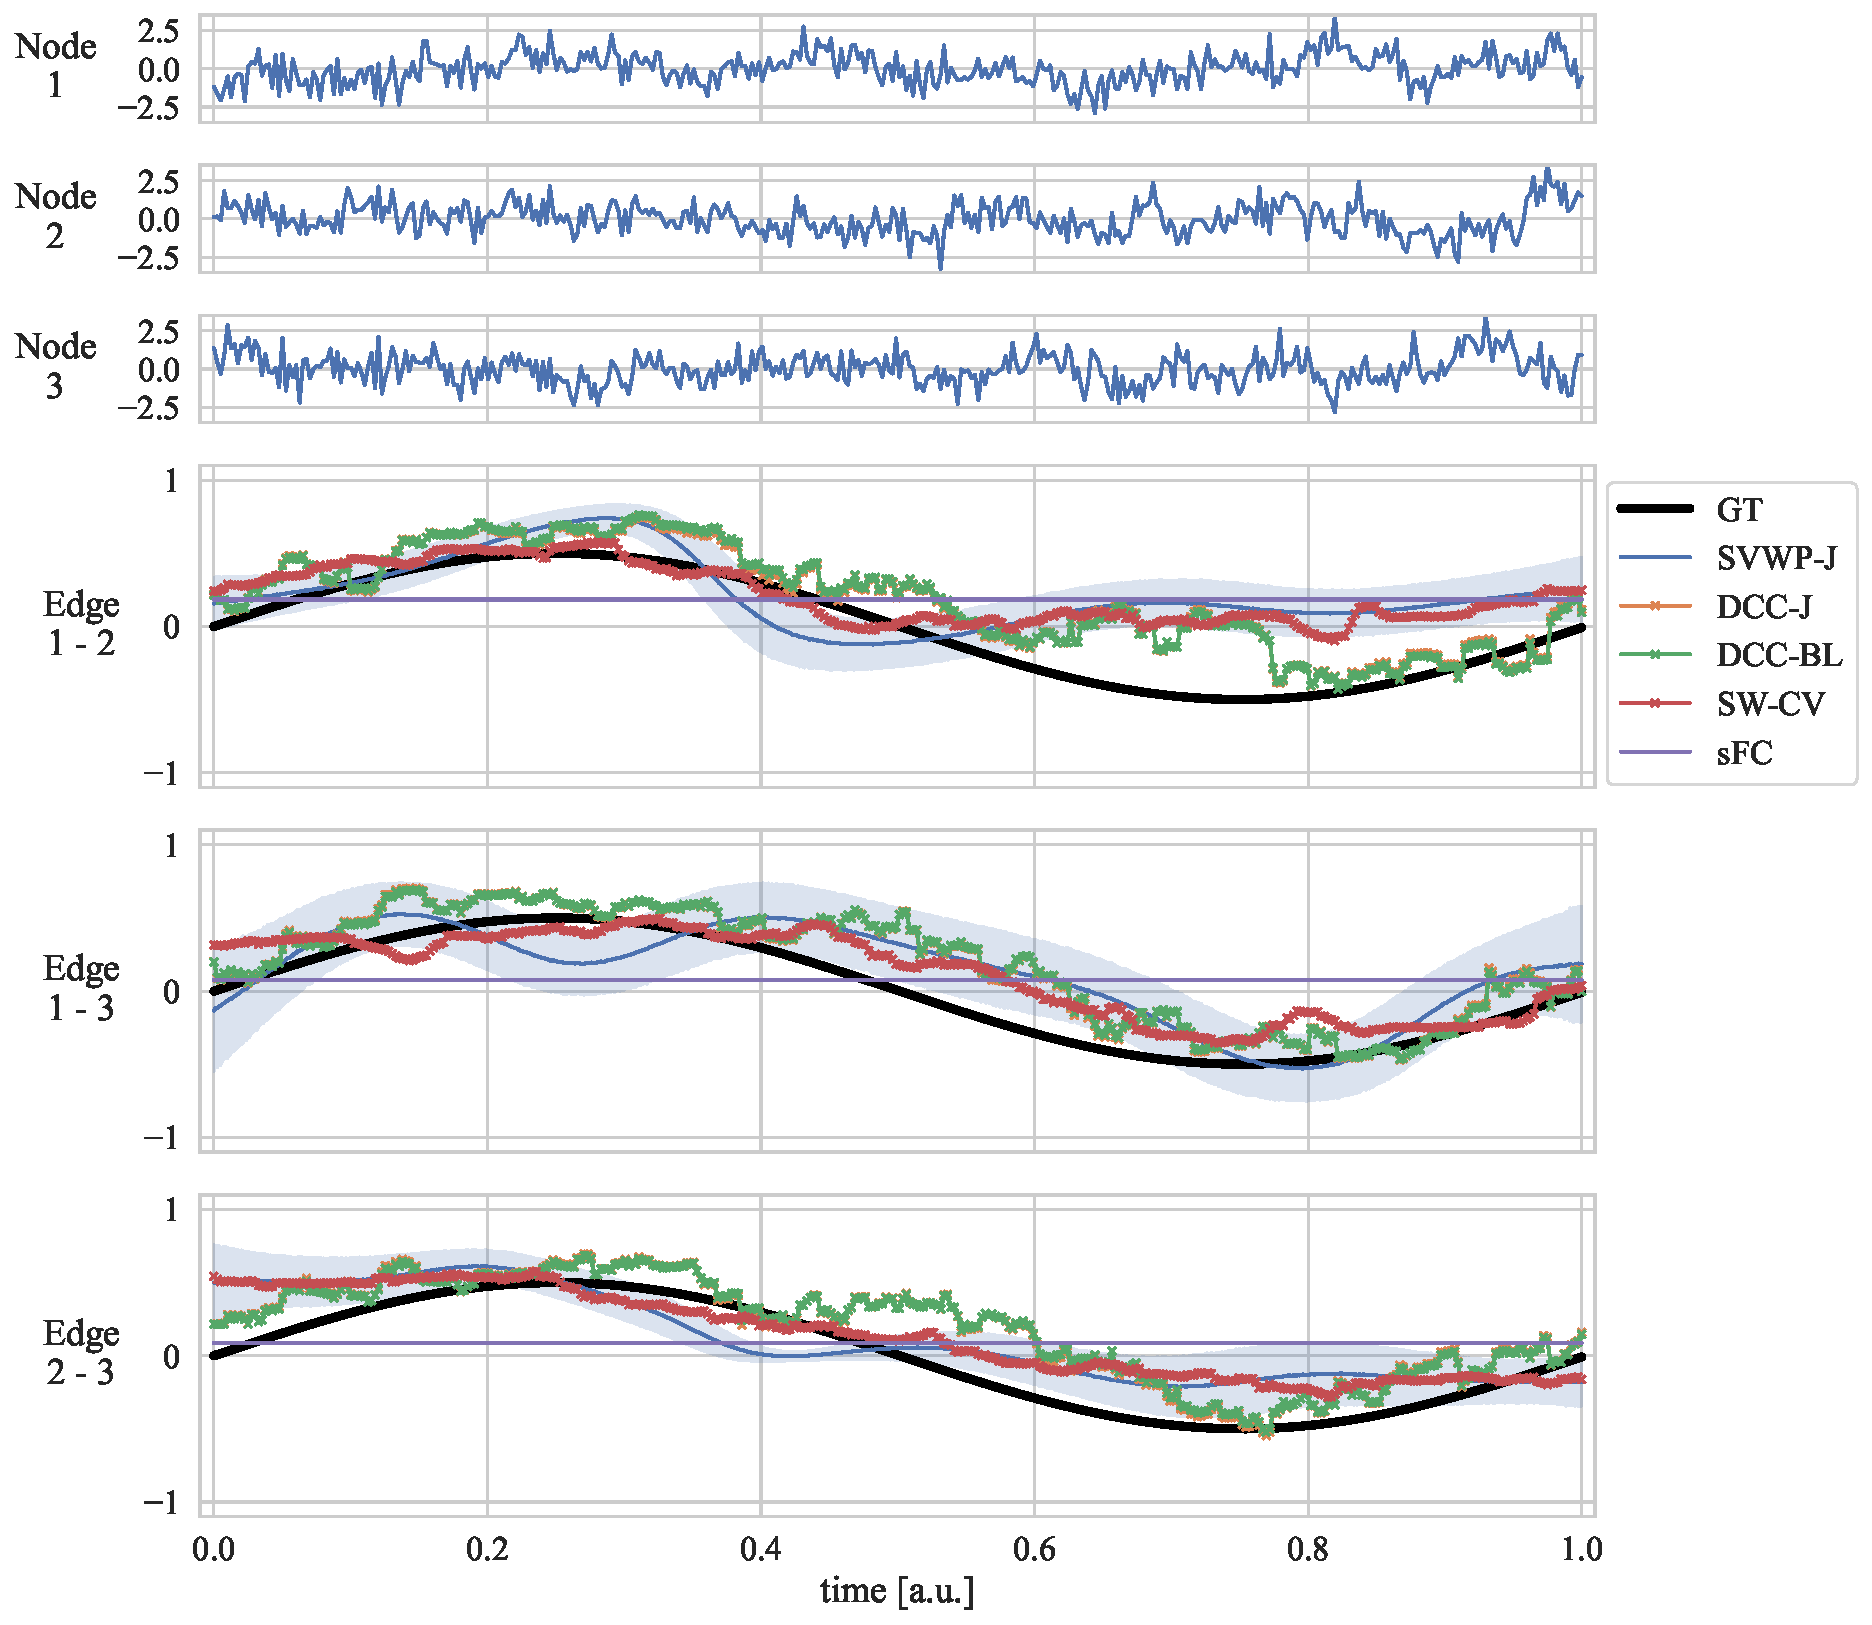
\includegraphics[width=\textwidth]{fig/sim/d3d/N0400_T0003/HCP_noise_snr_1/periodic_1_correlations}
  \caption{
    Model TVFC estimates on dense trivariate data for $N = 400$ data points.
    HCP noise with SNR of 1 added.
  }\label{fig:results-d3d-periodic-1-tvfc-predictions-snr-1}
\end{figure}


%%
\clearpage
\section{Simulations: Trivariate TVFC estimates}\label{ch:appendix-d3-tvfc-estimates}
%%


\begin{figure}[ht]
  \centering
  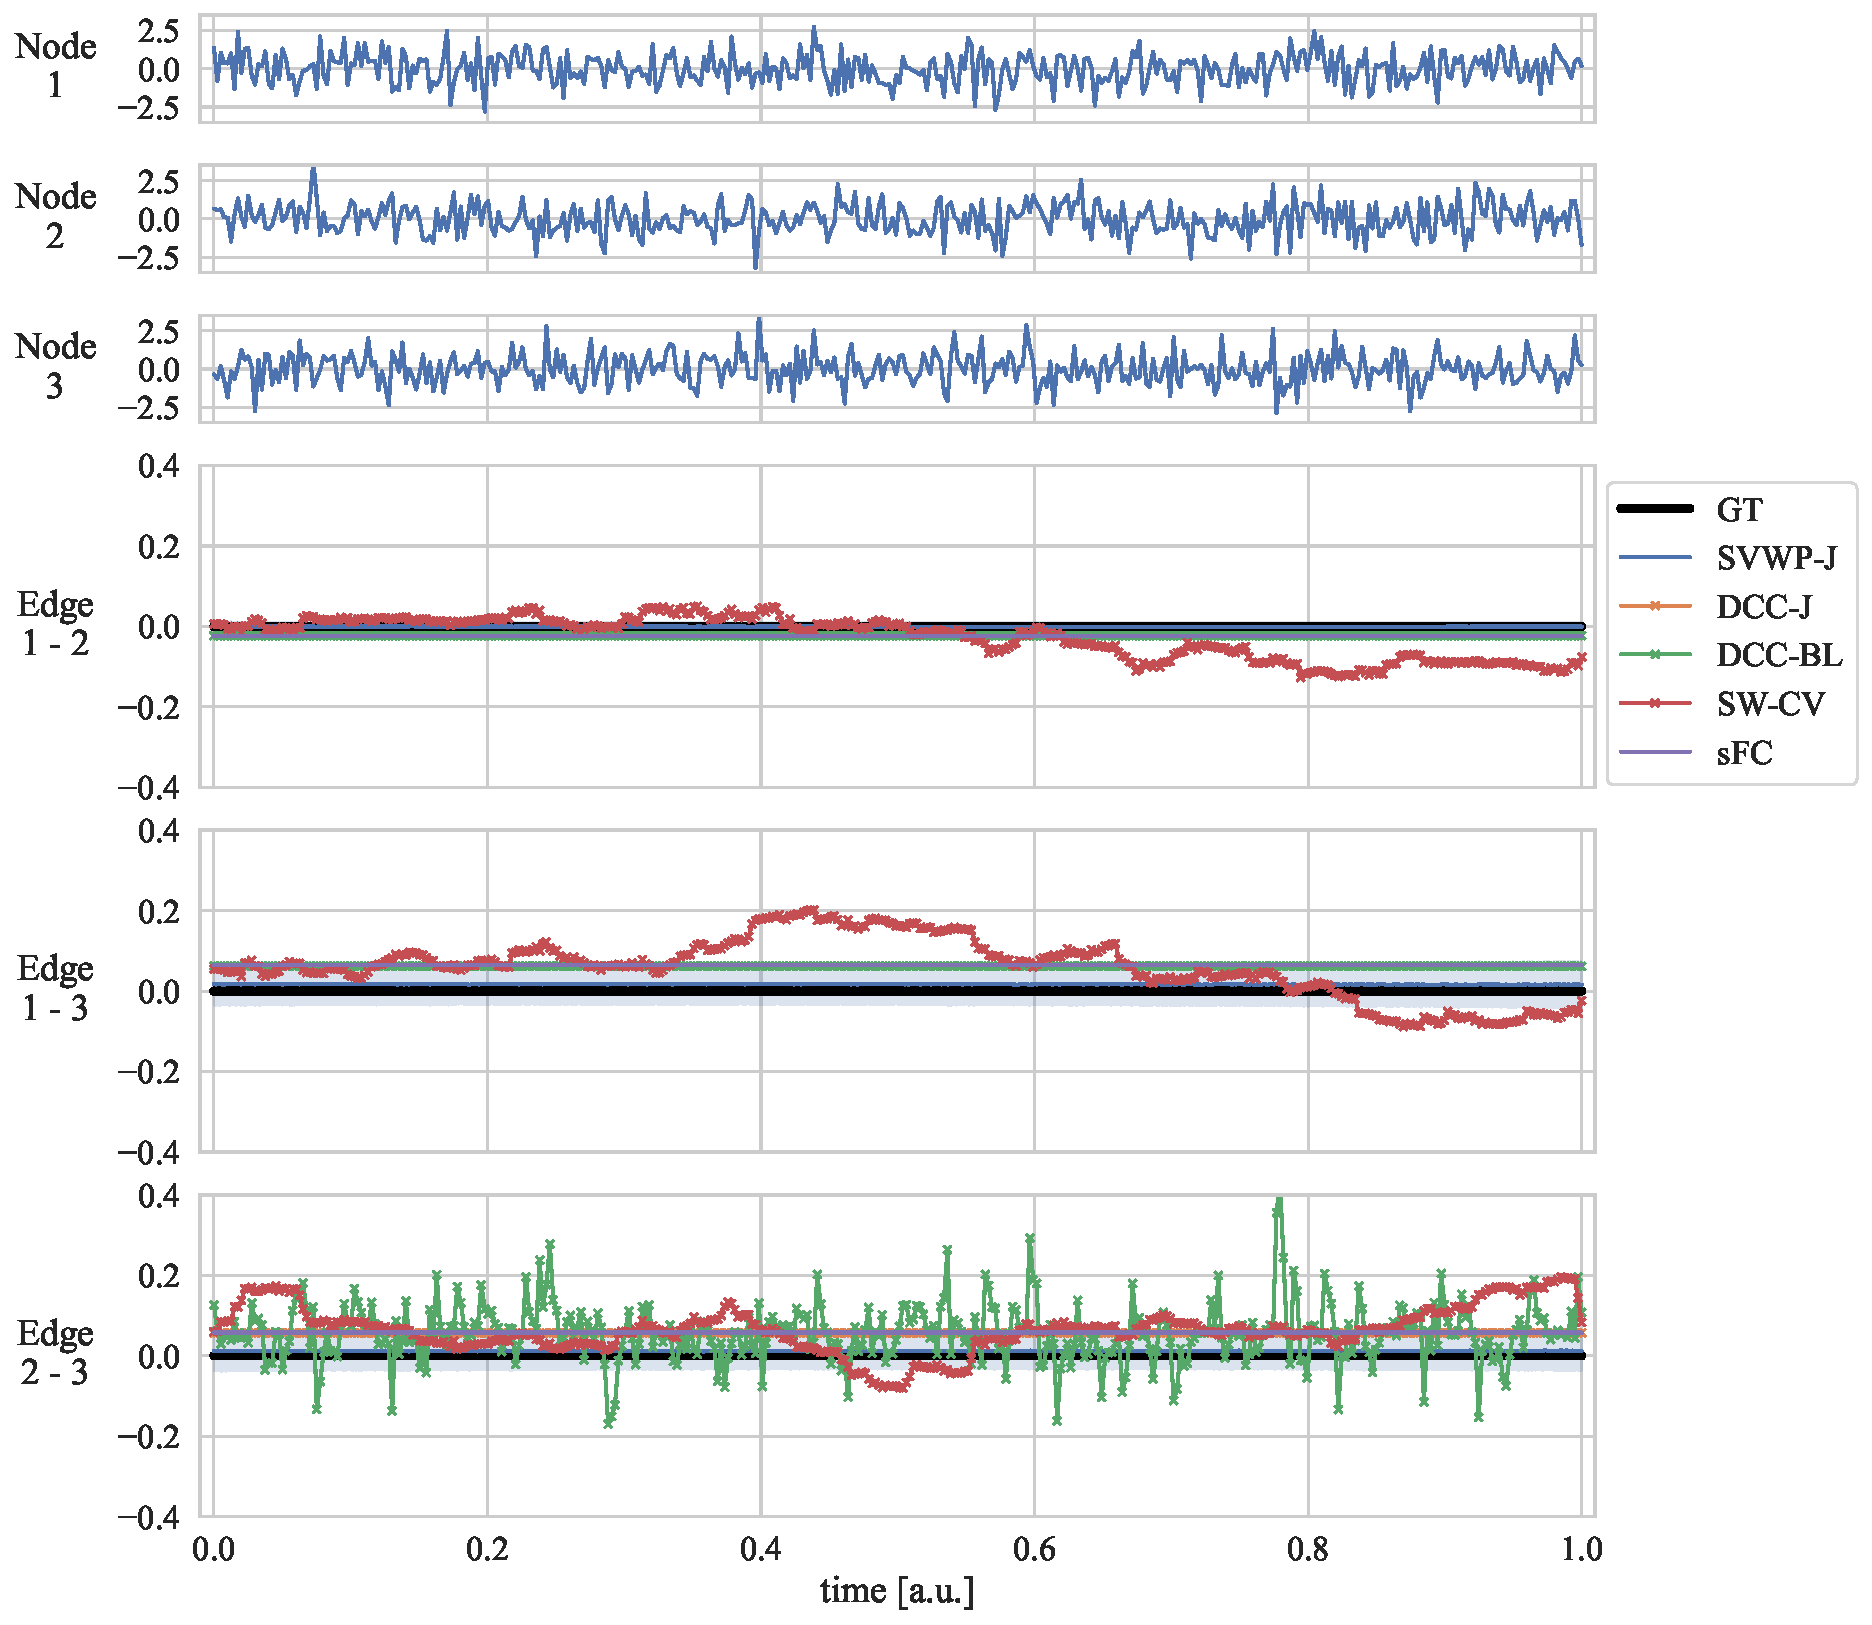
\includegraphics[width=\textwidth]{fig/sim/d3s/N0400_T0003/no_noise/null_correlations}
  \caption{
    Simulations benchmark single trial TVFC estimates for null covariance structure, for trivariate ($D = 3$) data for $N = 400$.
  }\label{fig:results-d3-no-noise-null-covariance}
\end{figure}


\begin{figure}[ht]
  \centering
  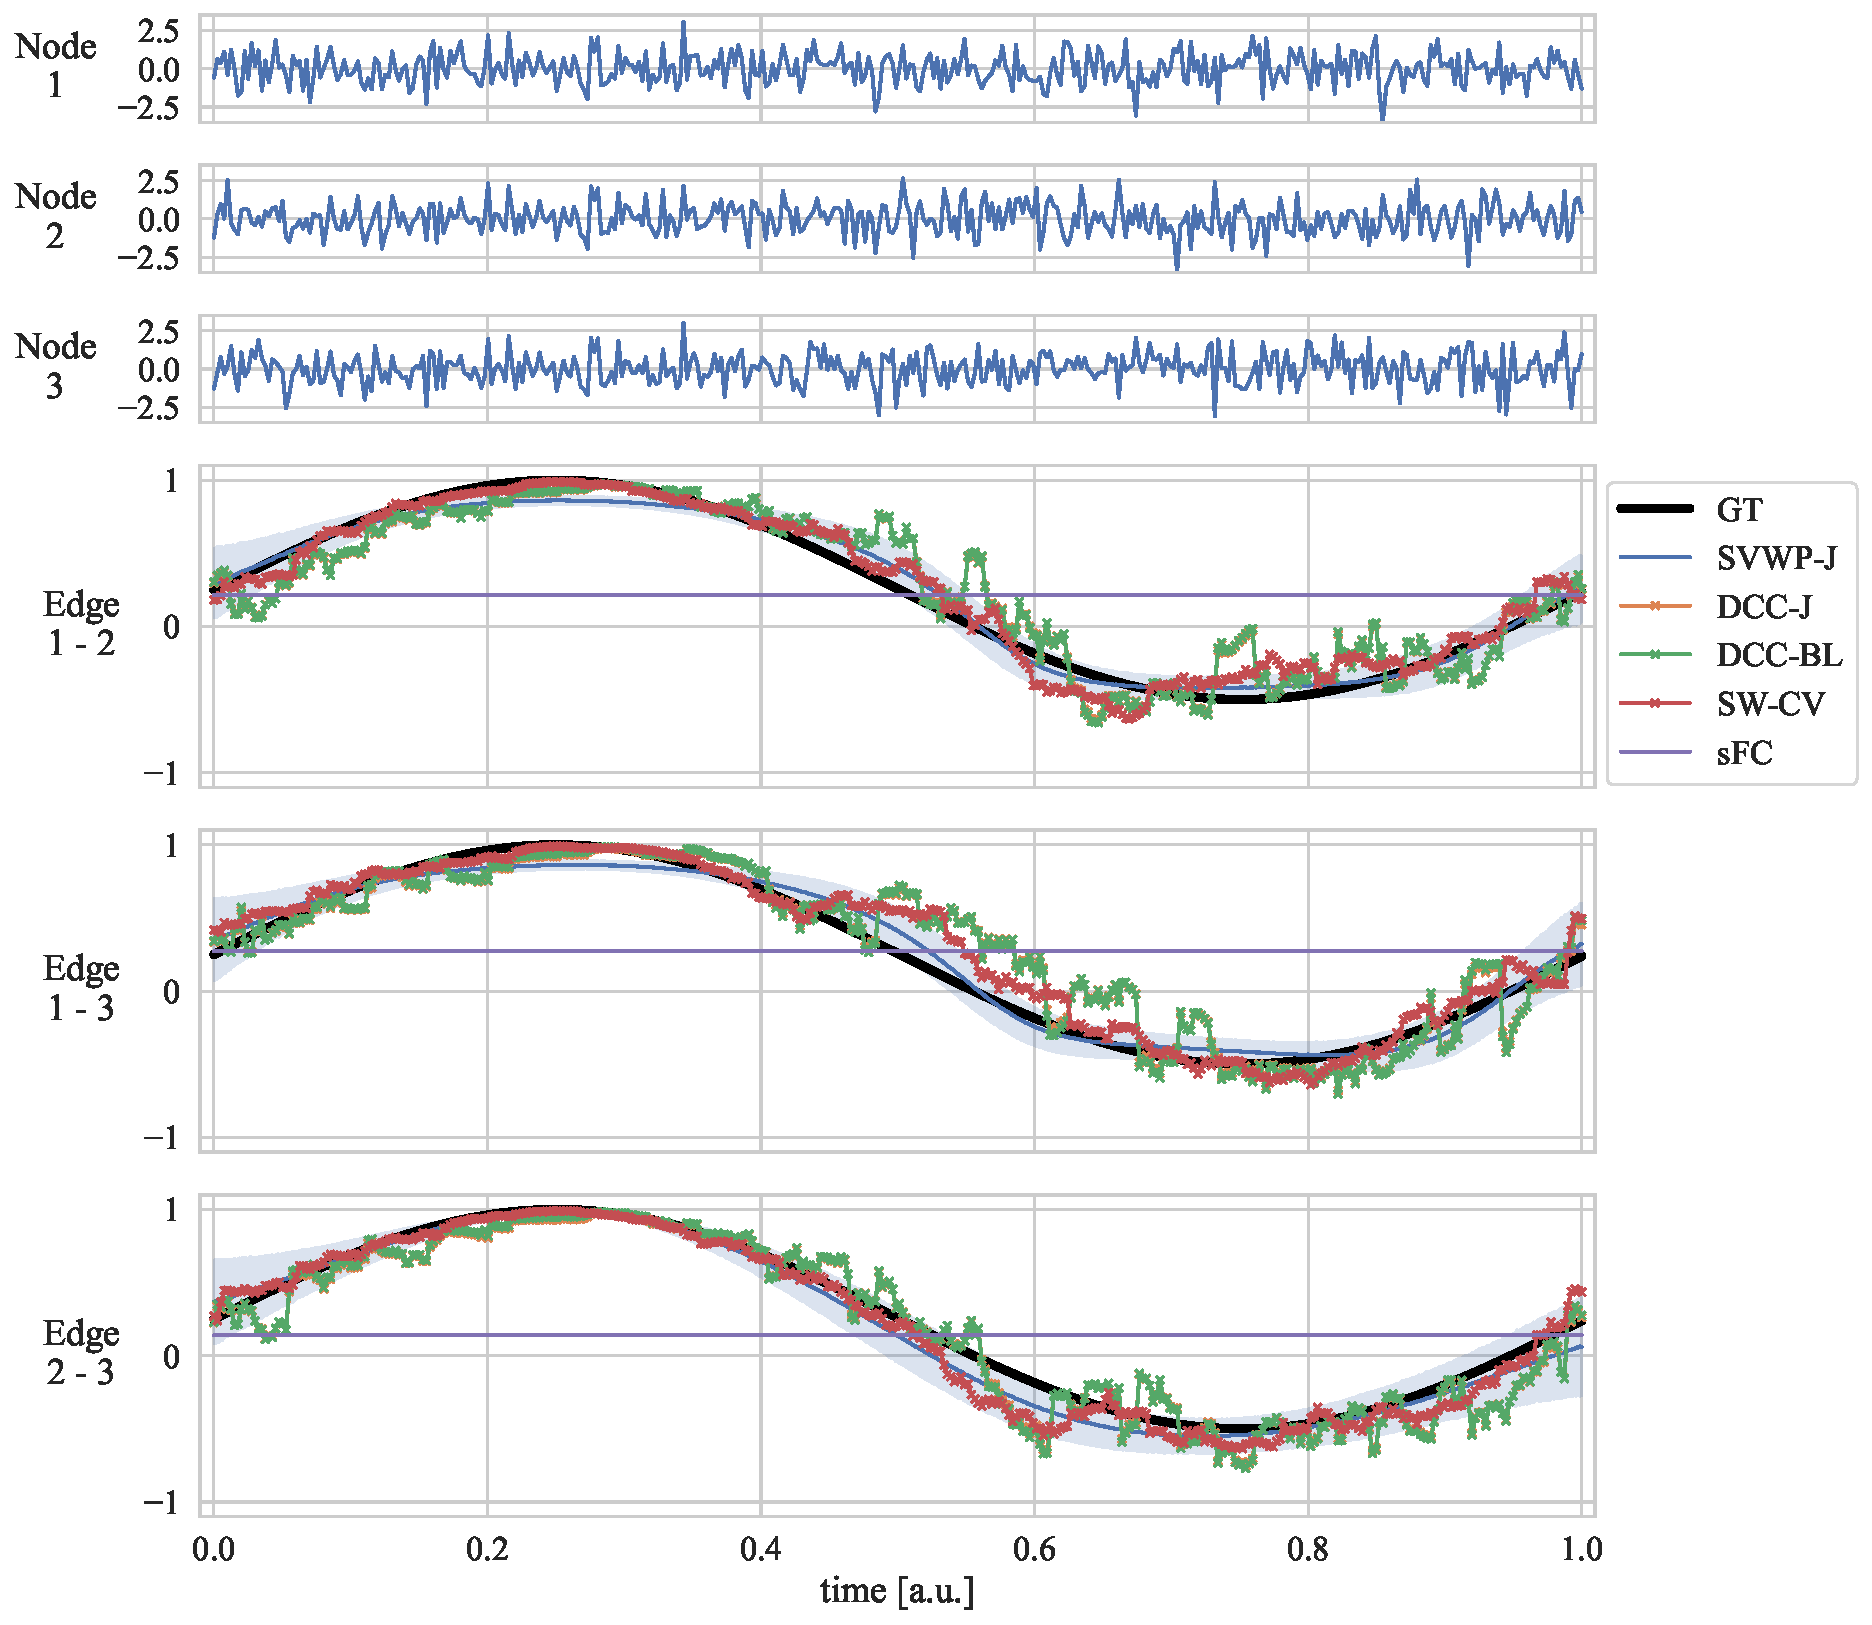
\includegraphics[width=\textwidth]{fig/sim/d3d/N0400_T0003/no_noise/periodic_1_correlations}
  \caption{
    Simulations benchmark single trial TVFC estimates for periodic (fast) covariance structure, for dense trivariate ($D = 3$) data for $N = 400$.
  }\label{fig:results-d3s-no-noise-periodic-3-covariance}
\end{figure}


\begin{figure}[ht]
  \centering
  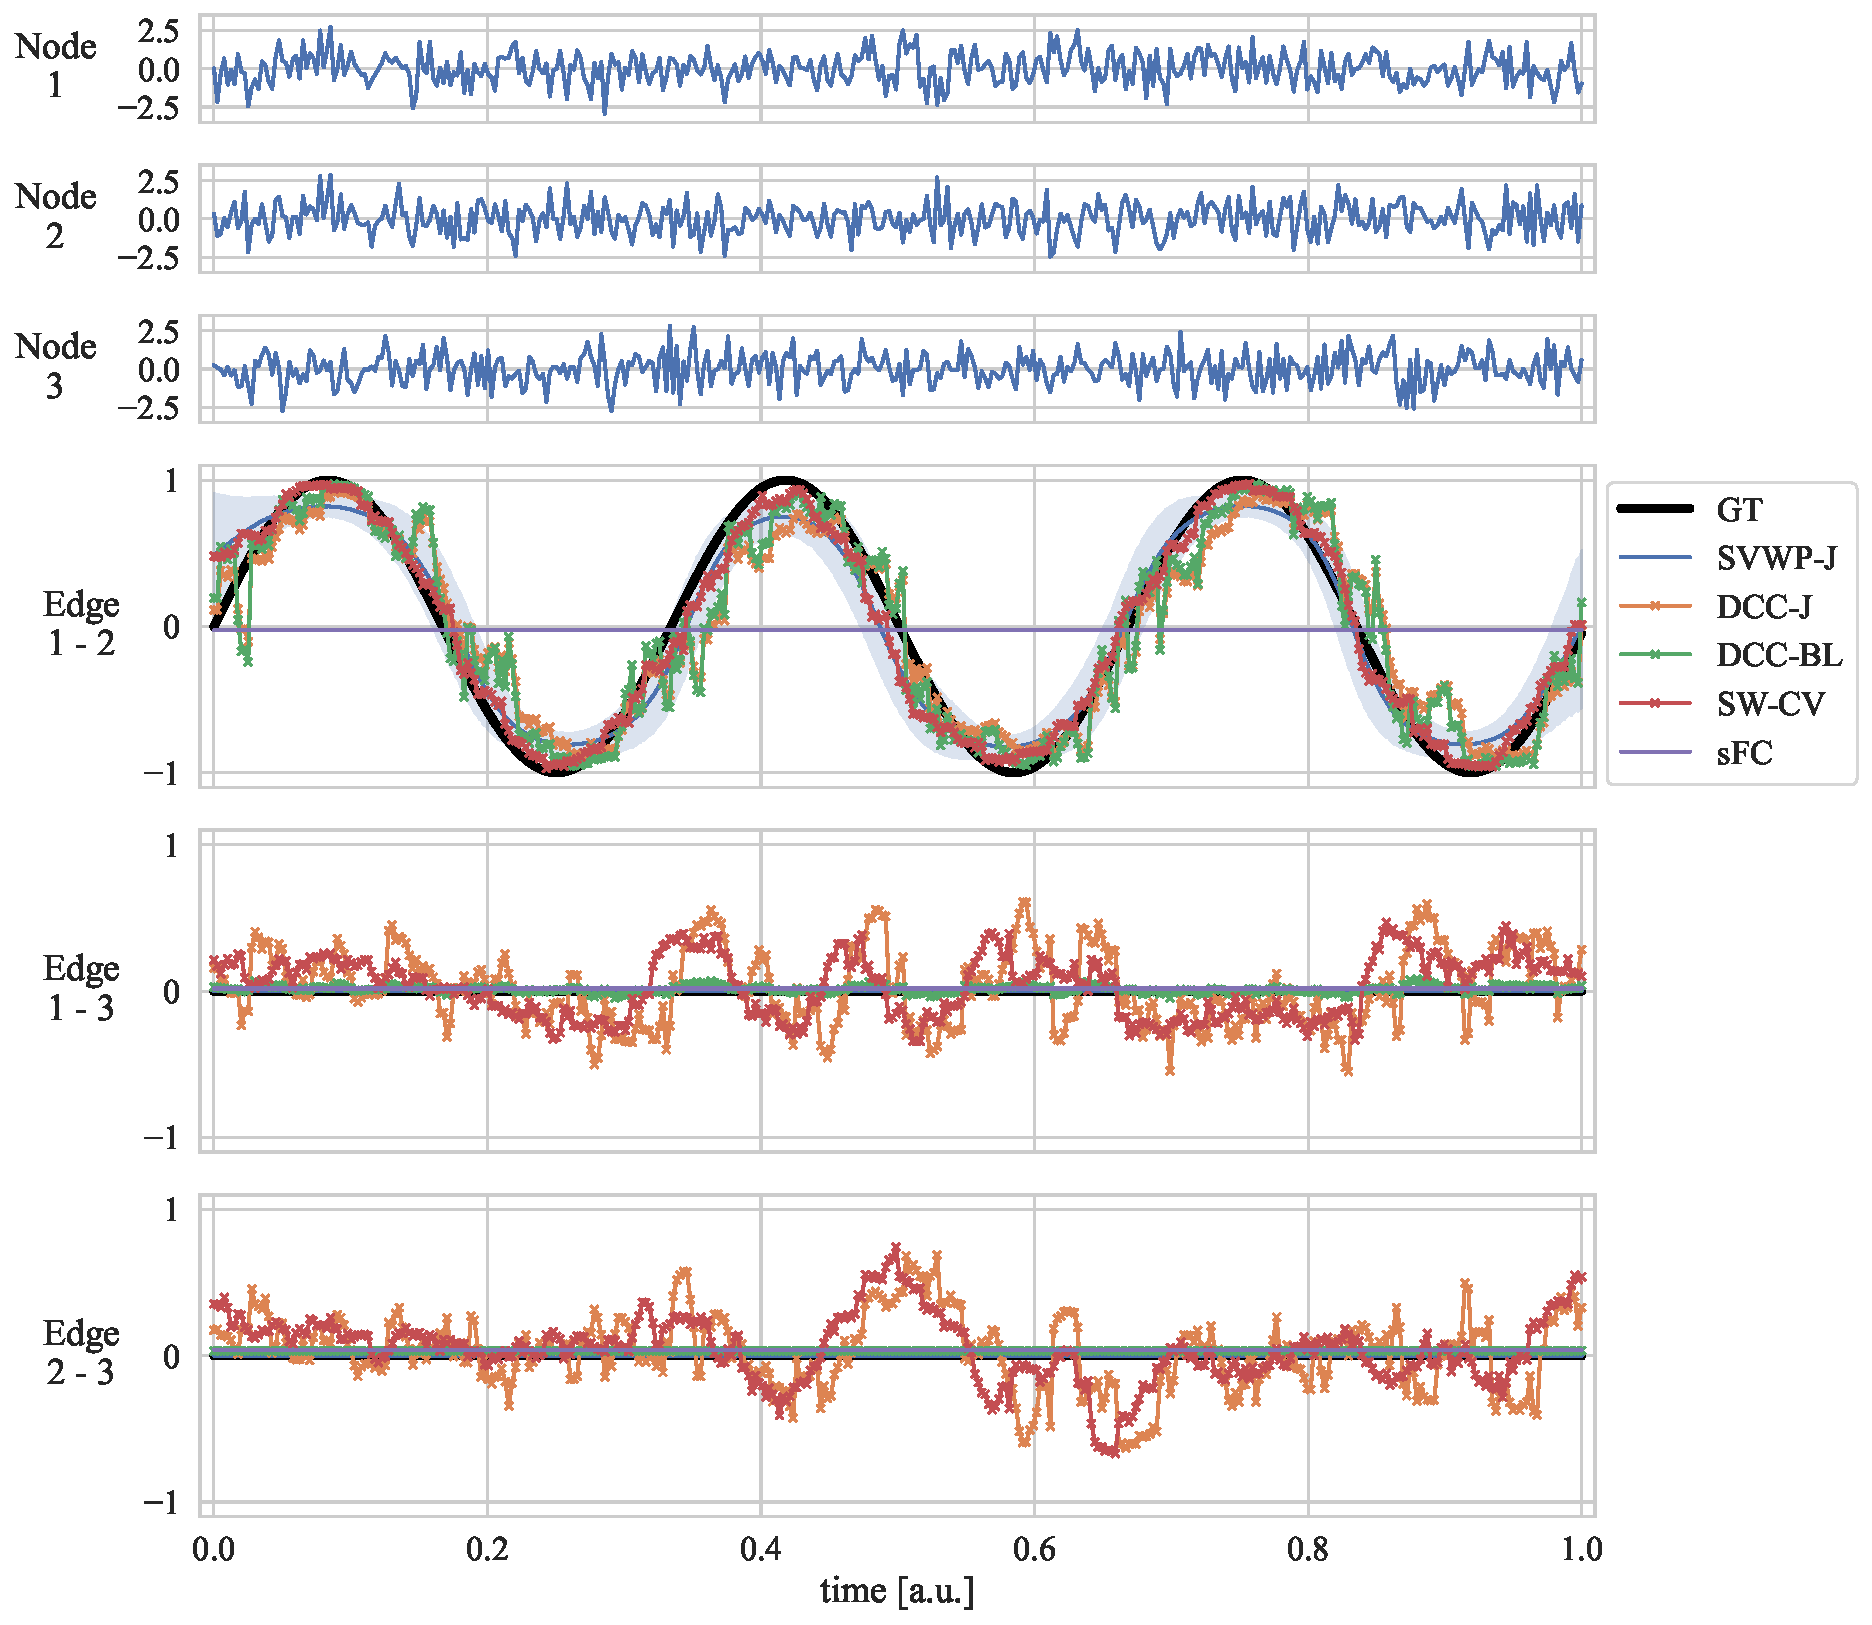
\includegraphics[width=\textwidth]{fig/sim/d3s/N0400_T0003/no_noise/periodic_3_correlations}
  \caption{
    Simulations benchmark single trial TVFC estimates for periodic (fast) covariance structure, for dense trivariate ($D = 3$) data for $N = 400$.
  }\label{fig:results-d3s-no-noise-stepwise-covariance}
\end{figure}


%%
\clearpage
\section{Simulations: More quantitative results}\label{appendix:sim-more-quantitative-results}
%%

%%
\subsection{Bivariate}
%%


\begin{figure}[ht]
  \centering
  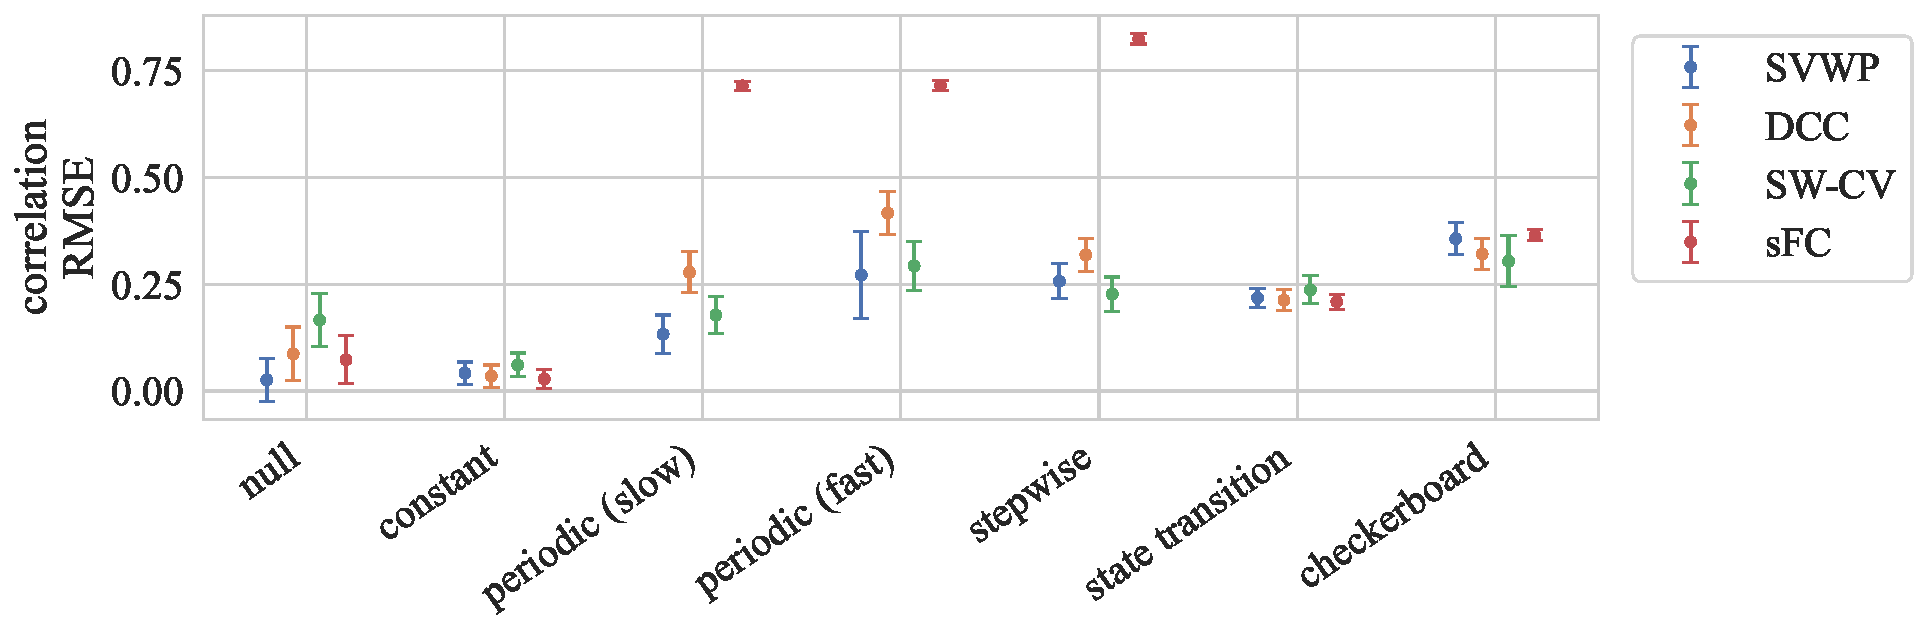
\includegraphics[width=0.84\textwidth]{fig/sim/d2/N0120_T0200/no_noise/correlation_RMSE}
  \caption{
    Simulations benchmark RMSE between model TVFC estimates and ground truth on all bivariate covariance structures with added rs-fMRI noise (SNR of 2) for $N = 120$.
    Means and standard deviations are shown across $T = 200$ trials.
  }\label{fig:results-sim-d2-120-no-noise-all-correlation-RMSE}
\end{figure}


\begin{figure}[ht]
  \centering
  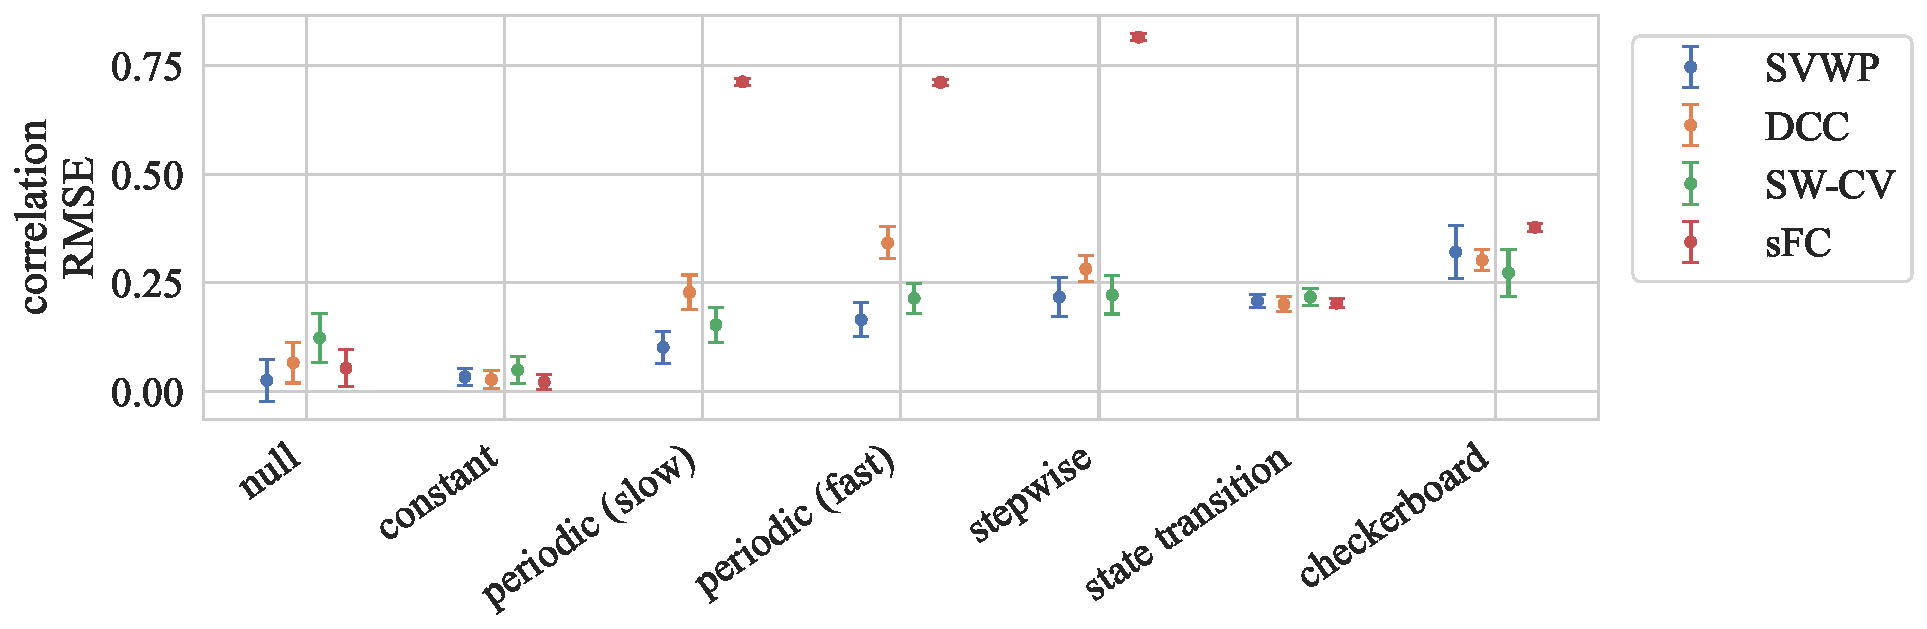
\includegraphics[width=0.84\textwidth]{fig/sim/d2/N0200_T0200/no_noise/correlation_RMSE}
  \caption{
    Simulations benchmark RMSE between model TVFC estimates and ground truth on all bivariate covariance structures with added rs-fMRI noise (SNR of 2) for $N = 200$.
    Means and standard deviations are shown across $T = 200$ trials.
  }\label{fig:results-sim-d2-200-no-noise-all-correlation-RMSE}
\end{figure}


\begin{figure}[ht]
  \centering
  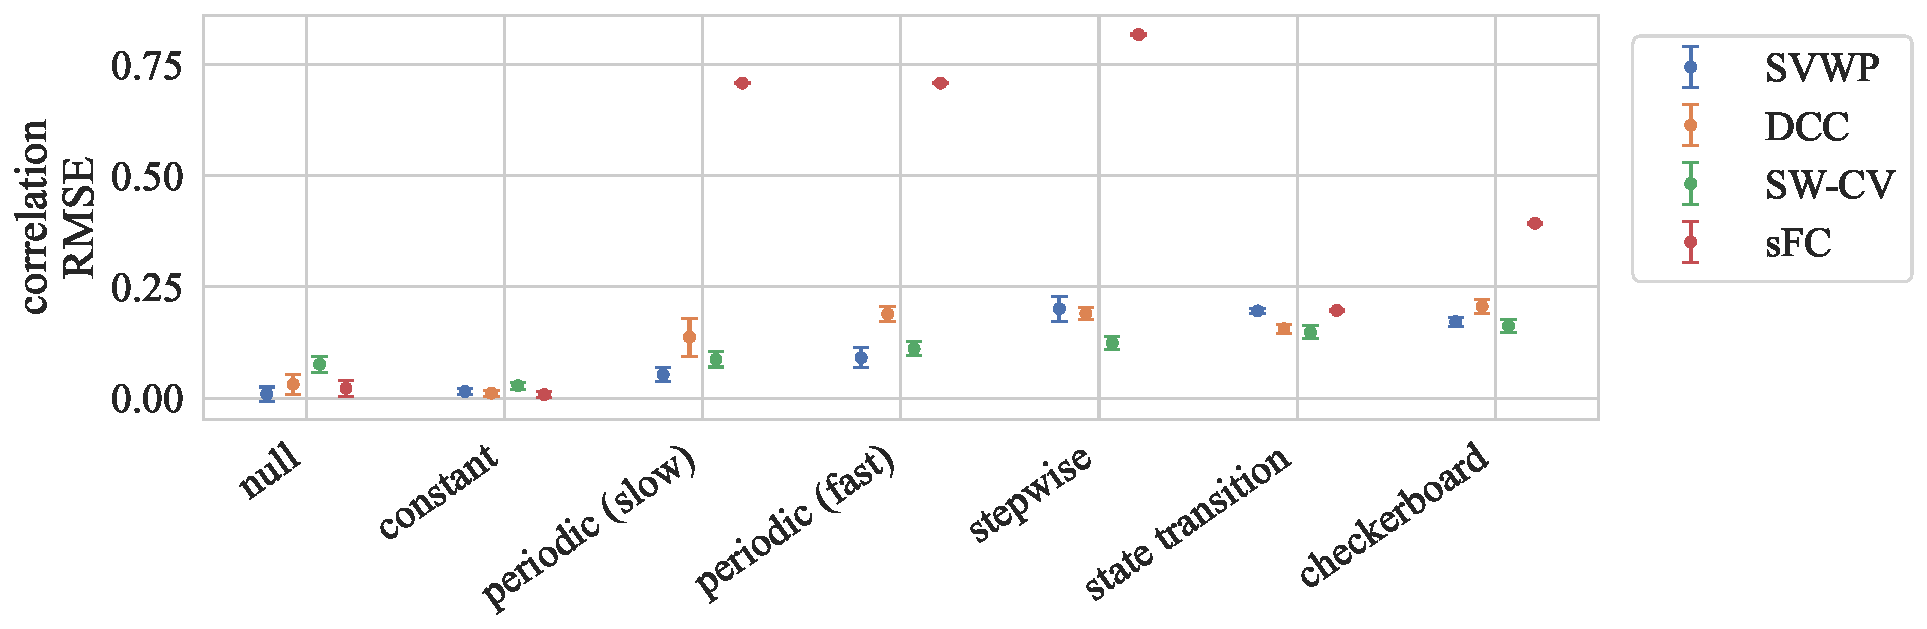
\includegraphics[width=0.84\textwidth]{fig/sim/d2/N1200_T0200/no_noise/correlation_RMSE}
  \caption{
    Simulations benchmark RMSE between model TVFC estimates and ground truth on all bivariate covariance structures with added rs-fMRI noise (SNR of 2) for $N = 1200$.
    Means and standard deviations are shown across $T = 200$ trials.
  }\label{fig:results-sim-d2-1200-no-noise-all-correlation-RMSE}
\end{figure}


%%
\clearpage
\subsection{Trivariate}
%%


\begin{figure}[ht]
  \centering
  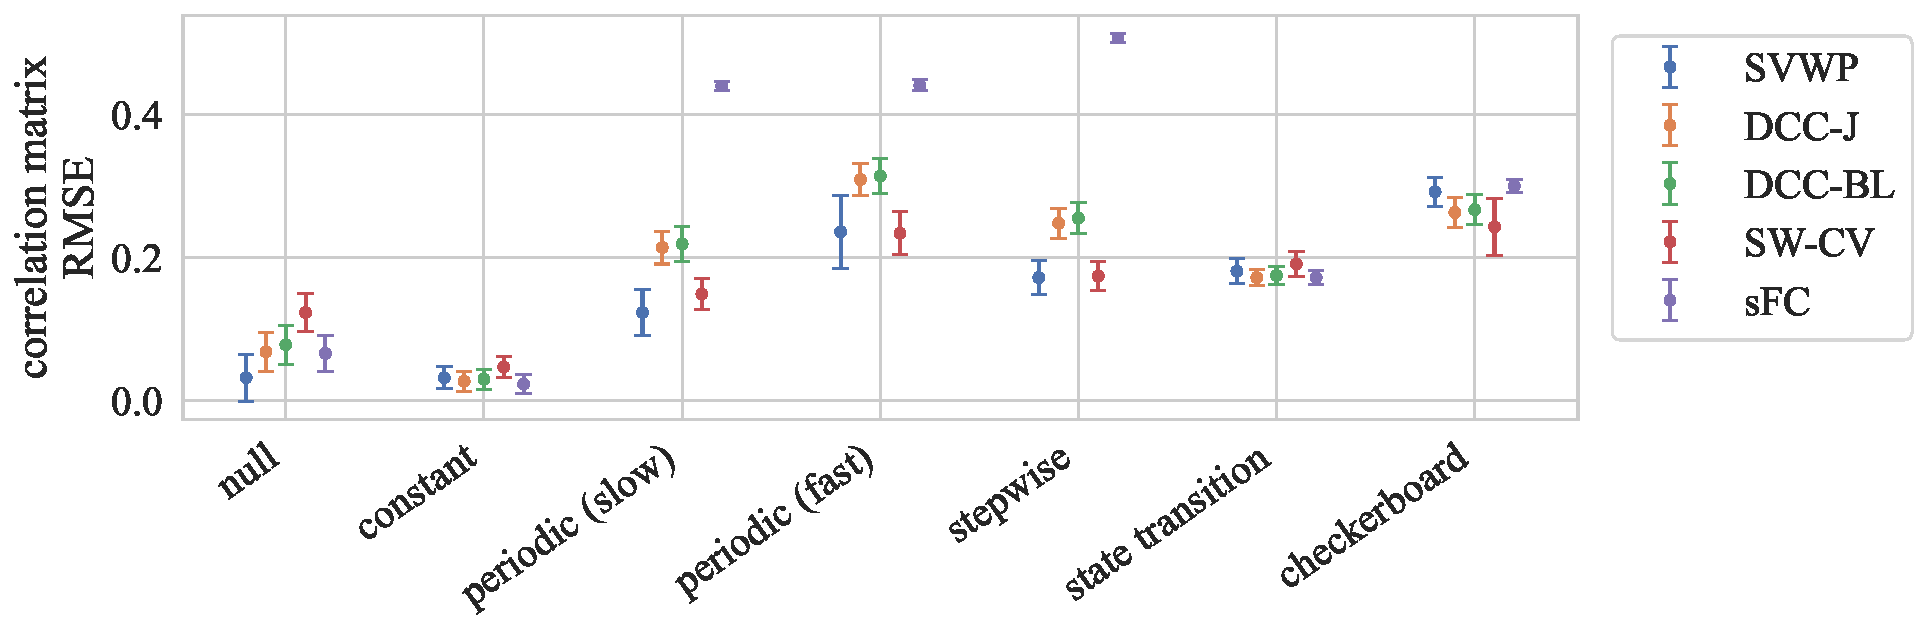
\includegraphics[width=0.84\textwidth]{fig/sim/d3d/N0120_T0200/no_noise/correlation_matrix_RMSE}
  \caption{
    Simulations benchmark RMSE between model TVFC estimates and ground truth on all dense trivariate covariance structures with added rs-fMRI noise (SNR of 2) for $N = 120$.
    Means and standard deviations are shown across $T = 200$ trials.
  }\label{fig:results-sim-d3d-120-no-noise-all-correlation-matrix-RMSE}
\end{figure}


\begin{figure}[ht]
  \centering
  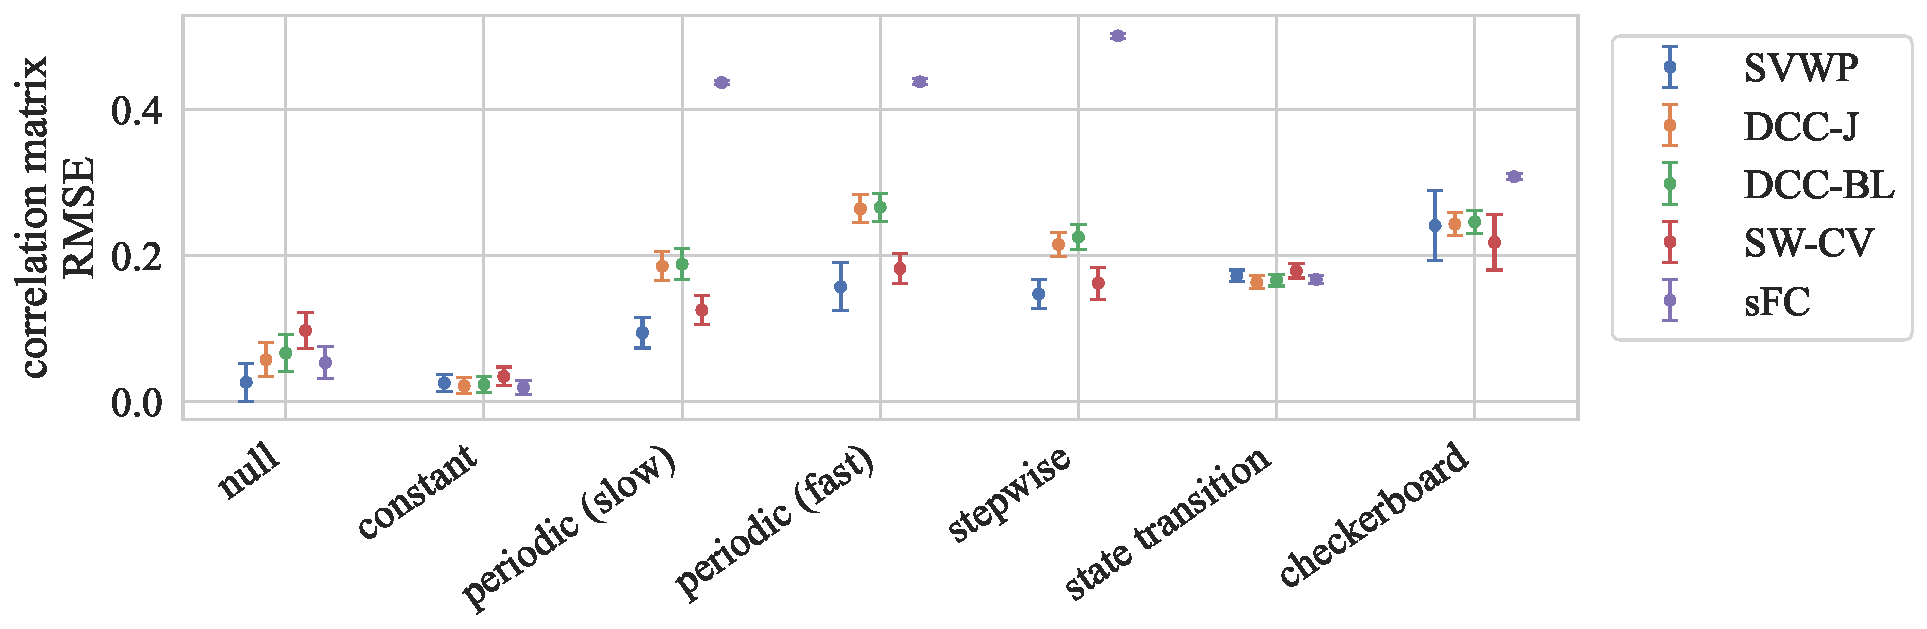
\includegraphics[width=0.84\textwidth]{fig/sim/d3d/N0200_T0200/no_noise/correlation_matrix_RMSE}
  \caption{
    Simulations benchmark RMSE between model TVFC estimates and ground truth on all dense trivariate covariance structures with added rs-fMRI noise (SNR of 2) for $N = 200$.
    Means and standard deviations are shown across $T = 200$ trials.
  }\label{fig:results-sim-d3d-200-no-noise-all-correlation-matrix-RMSE}
\end{figure}


\begin{figure}[ht]
  \centering
  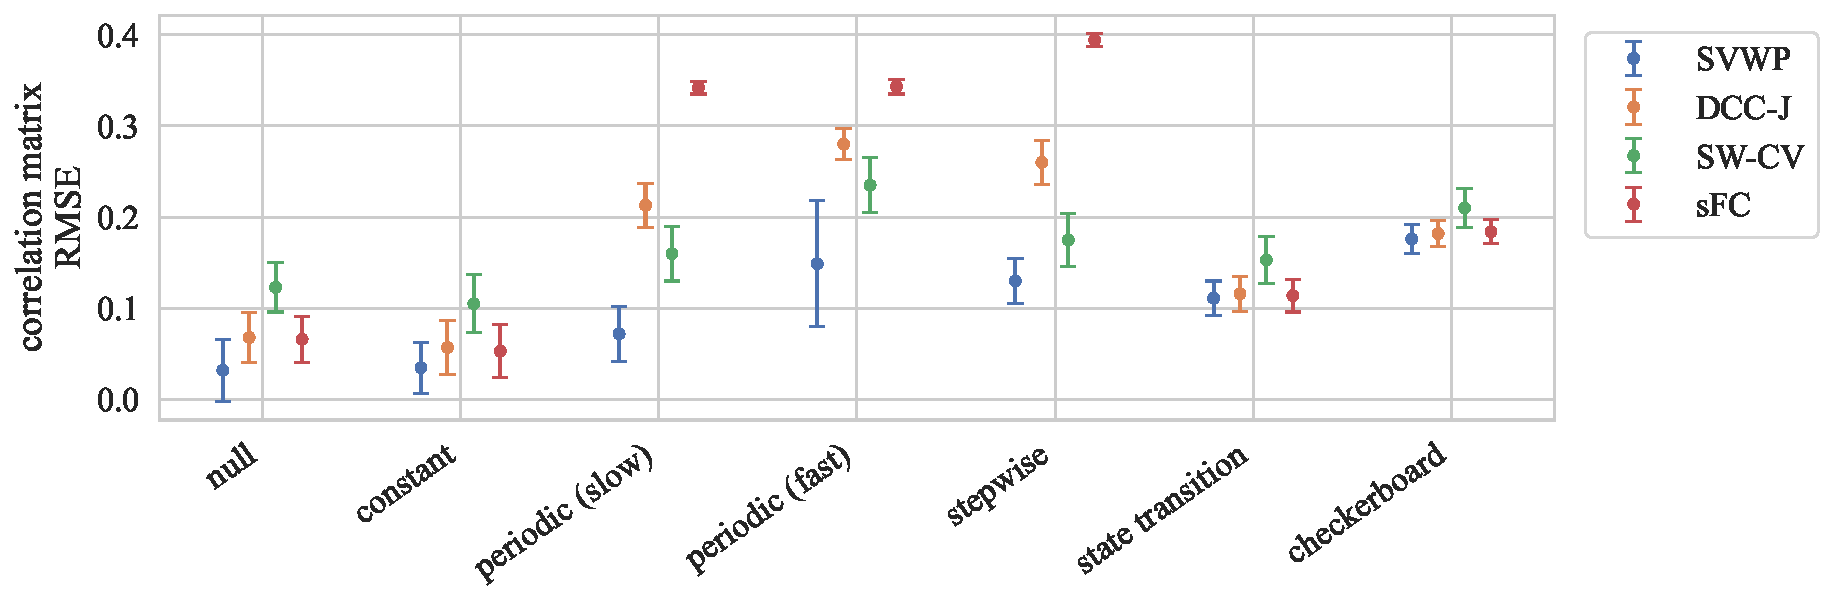
\includegraphics[width=0.84\textwidth]{fig/sim/d3s/N0120_T0200/no_noise/correlation_matrix_RMSE}
  \caption{
    Simulations benchmark RMSE between model TVFC estimates and ground truth on all sparse trivariate covariance structures with added rs-fMRI noise (SNR of 2) for $N = 120$.
    Means and standard deviations are shown across $T = 200$ trials.
  }\label{fig:results-sim-d3s-120-no-noise-all-correlation-matrix-RMSE}
\end{figure}


\begin{figure}[ht]
  \centering
  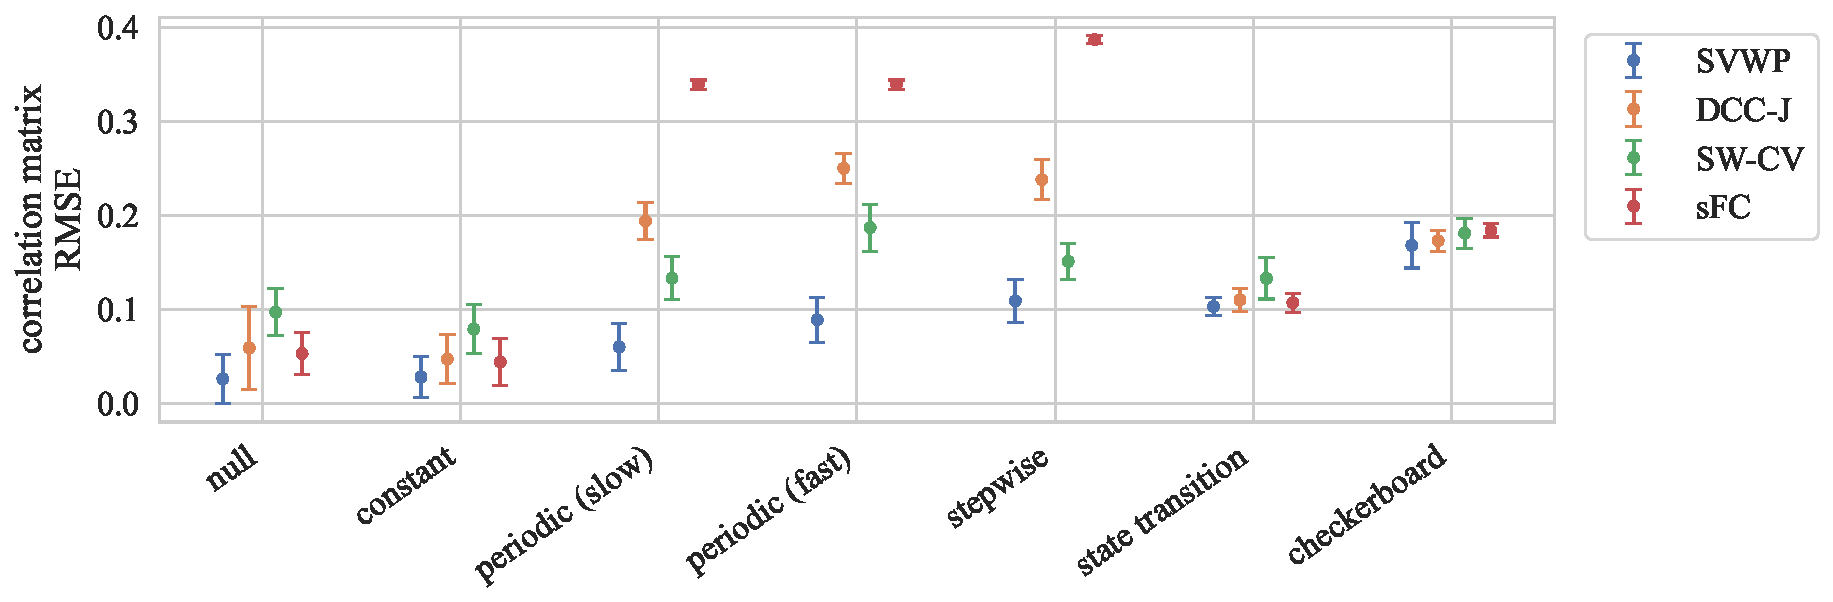
\includegraphics[width=0.84\textwidth]{fig/sim/d3s/N0200_T0200/no_noise/correlation_matrix_RMSE}
  \caption{
    Simulations benchmark RMSE between model TVFC estimates and ground truth on all sparse trivariate covariance structures with added rs-fMRI noise (SNR of 2) for $N = 200$.
    Means and standard deviations are shown across $T = 200$ trials.
  }\label{fig:results-sim-d3s-200-no-noise-all-correlation-matrix-RMSE}
\end{figure}


\clearpage
\section{HCP: Extra subject measure predictions}\label{appendix:hcp-more-results}
%%


\begin{figure}[h]
  \centering
  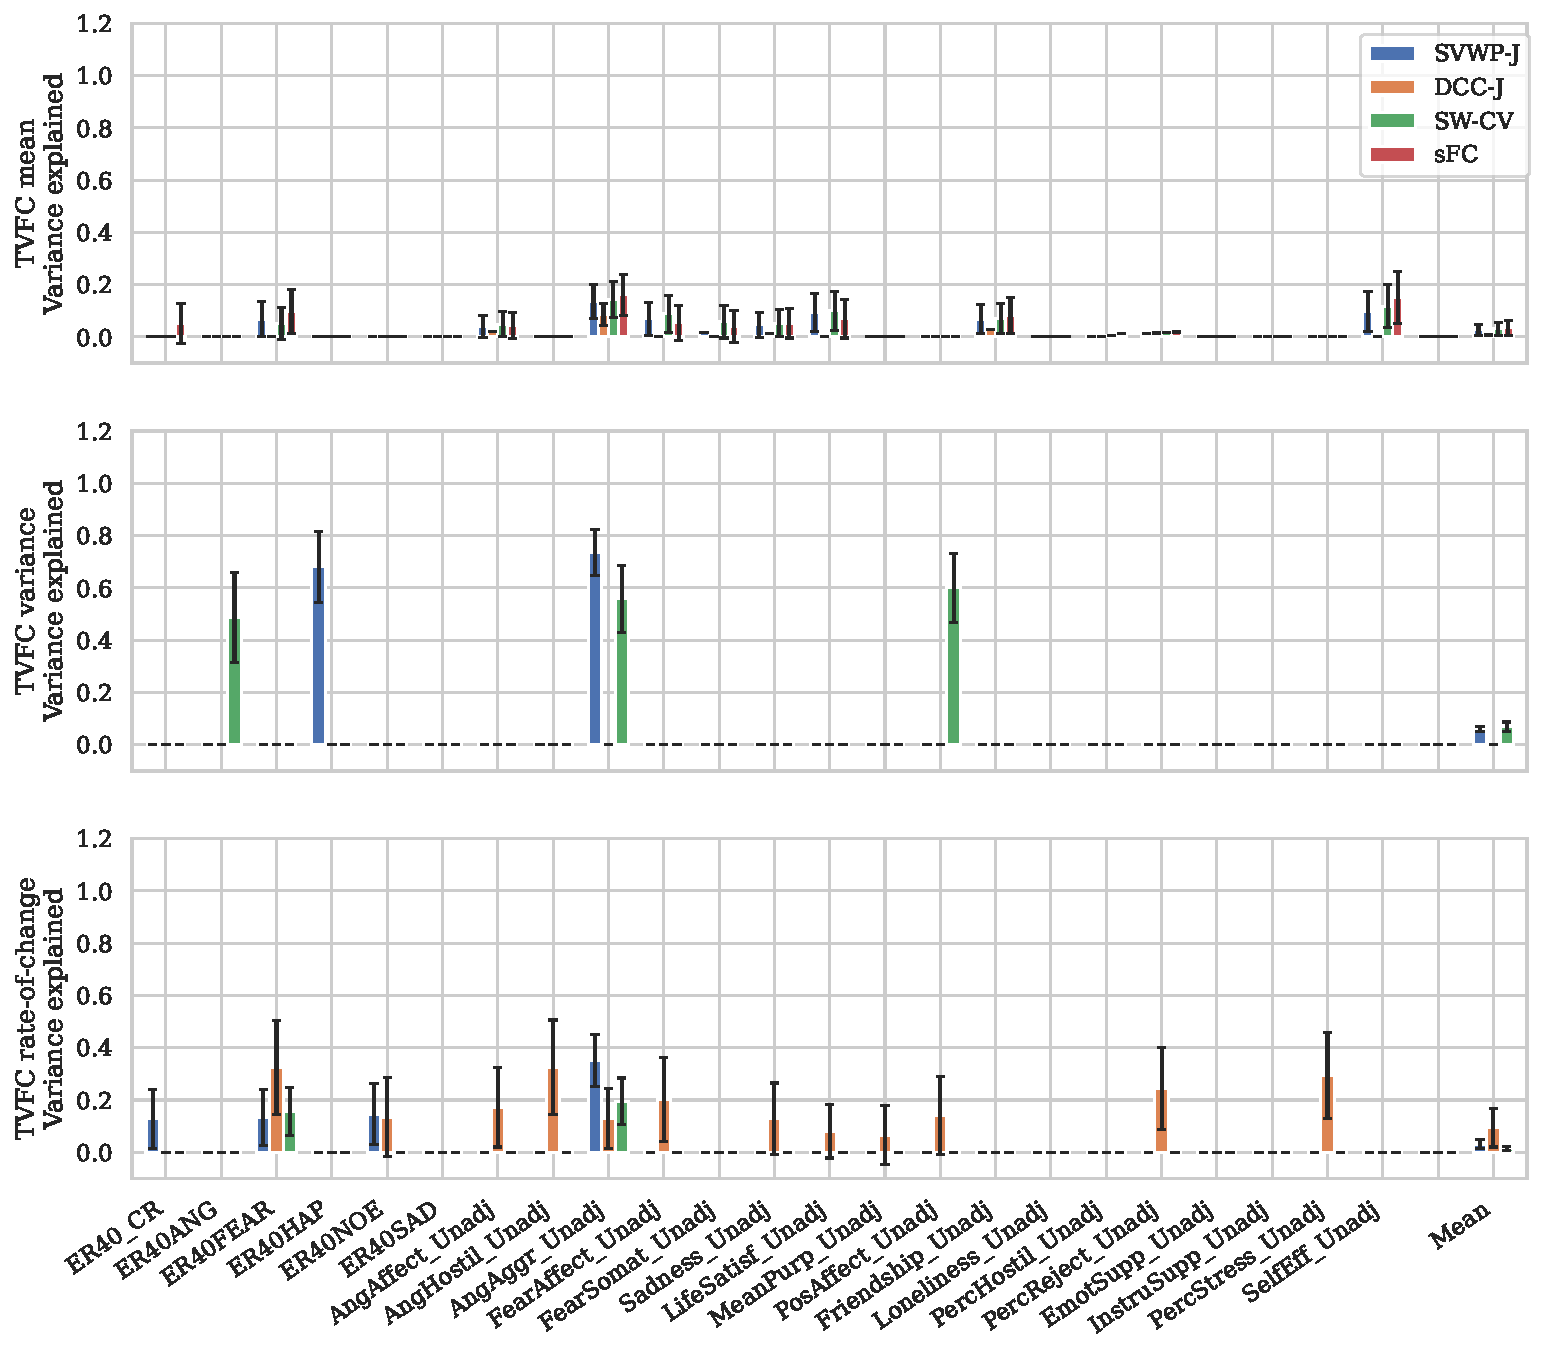
\includegraphics[width=\textwidth]{fig/hcp/d15/subject_measure_prediction/social-emotional/morphometricity_all_TVFC_summary_measures}
  \caption{
    HCP benchmark subject social-emotional measures prediction morphometricity scores (with standard error).
    Run on TVFC summary measures of mean (top), variance (middle), and rate-of-change (bottom row).
    sFC is added for reference to the TVFC mean plot.
  }\label{fig:results-subject-measures-prediction-social-emotional}
\end{figure}


\begin{figure}[h]
  \centering
  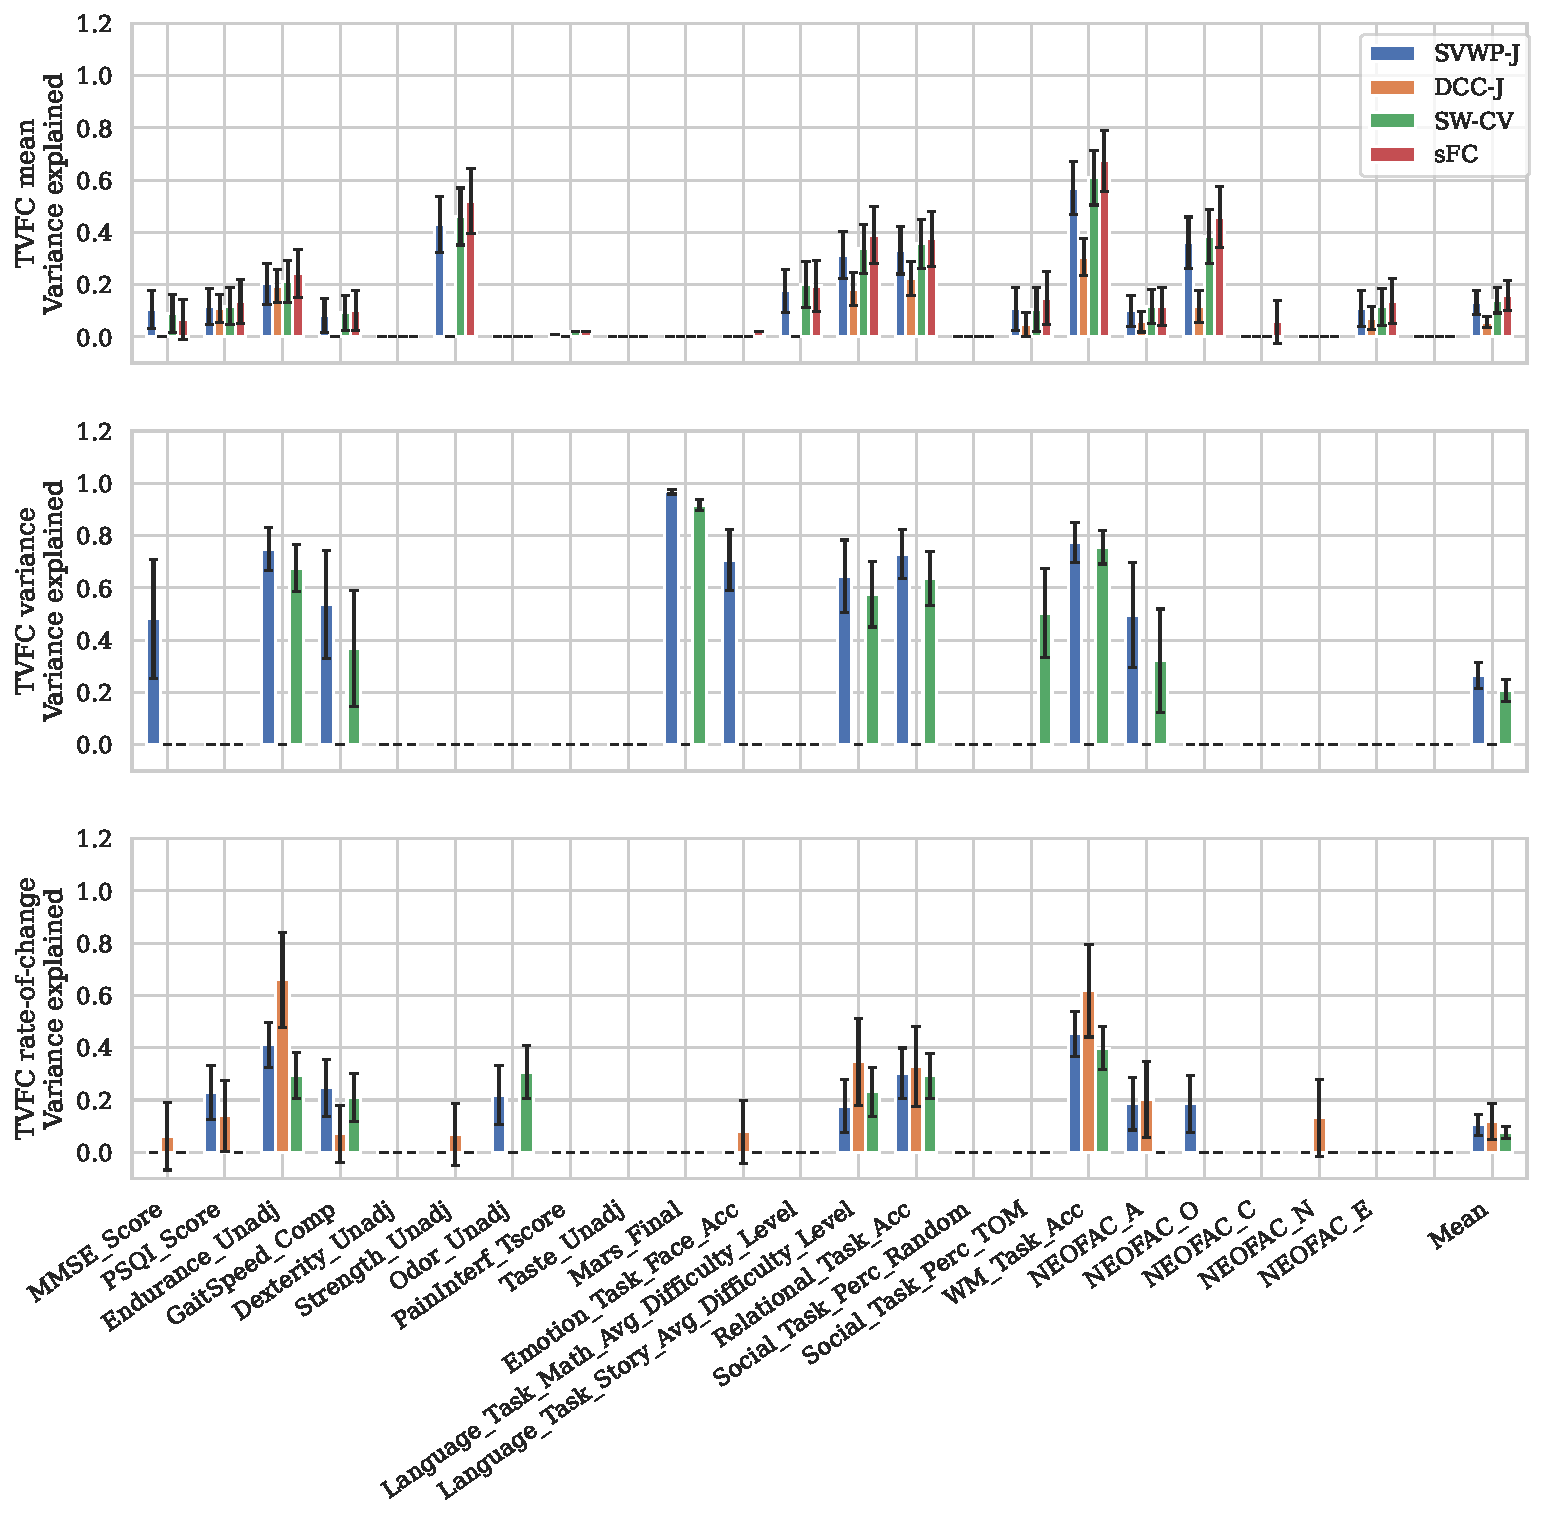
\includegraphics[width=\textwidth]{fig/hcp/d15/subject_measure_prediction/other/morphometricity_all_TVFC_summary_measures}
  \caption{
    HCP benchmark subject other measures prediction morphometricity scores (with standard error).
    Run on TVFC summary measures of mean (top), variance (middle), and rate-of-change (bottom row).
    sFC is added for reference to the TVFC mean plot.
  }\label{fig:results-subject-measures-prediction-other}
\end{figure}


%%
\clearpage
\section{HCP: Brain states}\label{appendix:hcp-brain-states}
%%


\begin{figure}[ht]
  \centering
  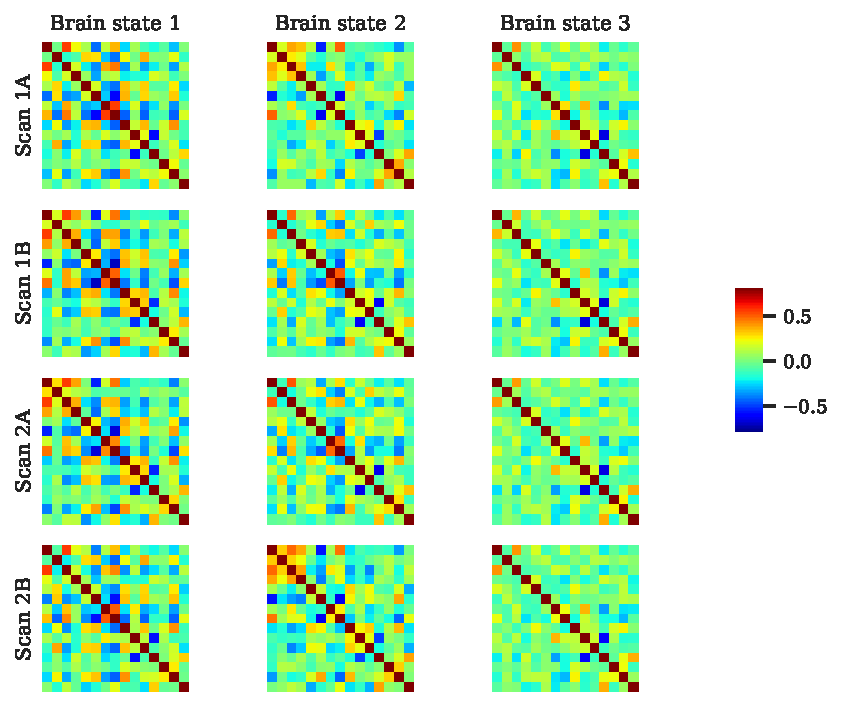
\includegraphics[width=\textwidth, trim={0.0cm 0cm 0.0cm 0cm}, clip]{fig/hcp/d15/brain_states/k03/brain_states_SVWP_joint}
  \caption{
    Brain states extracted from SVWP TVFC estimates on HCP data ($D = 15$ time series).
    Brain states across the four scans look very similar.
  }\label{fig:hcp-results-brain-states-svwp}
\end{figure}


\begin{figure}[ht]
  \centering
  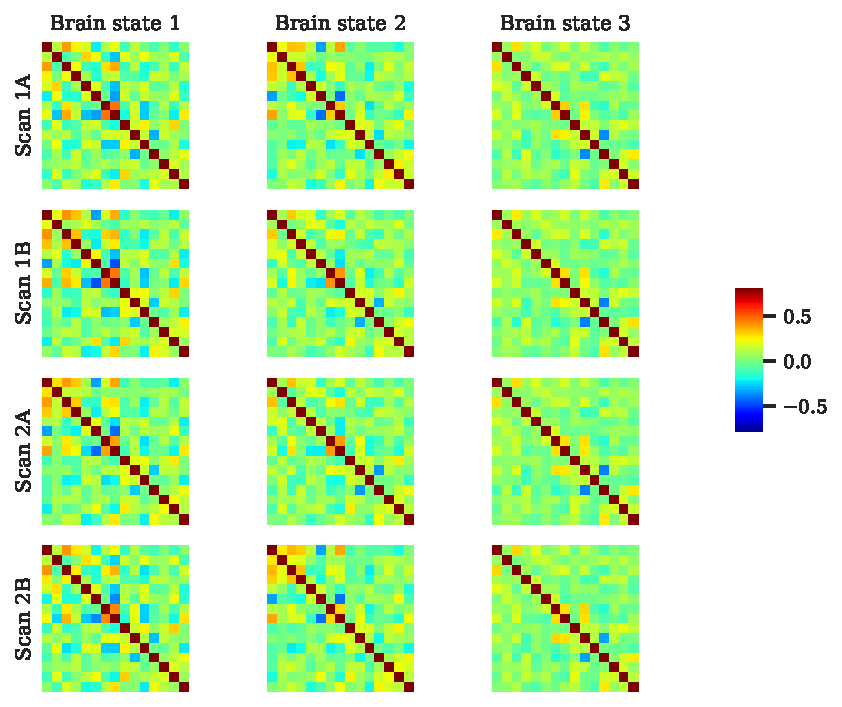
\includegraphics[width=\textwidth, trim={0.0cm 0cm 0.0cm 0cm}, clip]{fig/hcp/d15/brain_states/k03/brain_states_DCC_joint}
  \caption{
    Brain states extracted from DCC TVFC estimates on HCP data ($D = 15$ time series).
    Brain states are low contrast in general, and the four scans look very similar.
    This aligns with our intuition when looking at the DCC model predictions.
  }\label{fig:hcp-results-brain-states-dcc}
\end{figure}


\begin{figure}[ht]
  \centering
  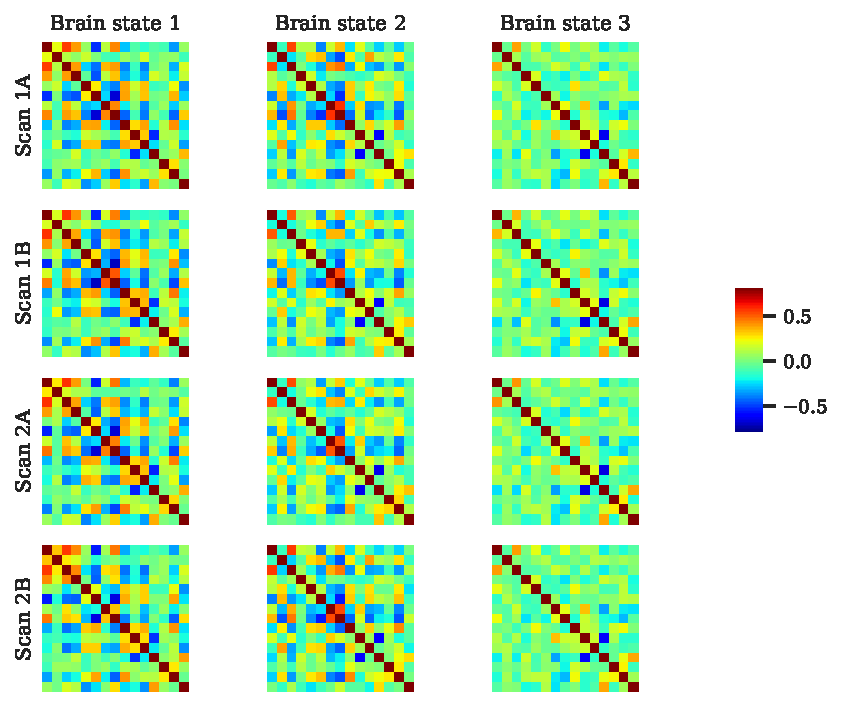
\includegraphics[width=\textwidth, trim={0.0cm 0cm 0.0cm 0cm}, clip]{fig/hcp/d15/brain_states/k03/brain_states_SW_cross_validated}
  \caption{
    Brain states extracted from SW-CV TVFC estimates on HCP data ($D = 15$ time series).
  }\label{fig:hcp-results-brain-states-sw-cv}
\end{figure}
